\documentclass{sadhana}

%% packages suggested by the Sadhana sample file
\usepackage{graphicx,amsmath,bm}
%% additional standard packages
\usepackage{booktabs,multirow,array,amssymb}
\usepackage{algorithm}
\usepackage[noend]{algpseudocode}
\usepackage[hidelinks]{hyperref}

\newcommand{\algname}{ArchTree}
\newcommand{\rmg}{ArchTree-RMG}
\newcommand{\pts}{\,pt}
\renewcommand{\algorithmicrequire}{\textbf{Input:}}
\renewcommand{\algorithmicensure}{\textbf{Output:}}
%% float placement for a two-column paper with many full-width figures
\setcounter{topnumber}{3}\setcounter{dbltopnumber}{3}\setcounter{totalnumber}{4}
\renewcommand{\topfraction}{0.9}\renewcommand{\dbltopfraction}{0.9}
\renewcommand{\textfraction}{0.1}\renewcommand{\floatpagefraction}{0.8}\renewcommand{\dblfloatpagefraction}{0.8}
\setlength{\emergencystretch}{1.5em}
%% list of symbols: same layout as the class, second column allowed to wrap
\renewenvironment{nomenclature}{\vskip 6pt\noindent{\textbf{Nomenclature}}\par\vskip 4pt\footnotesize\setlength{\parskip}{0.6pt}}{\par\vskip 6pt}
\newcommand{\nom}[2]{\par\noindent\hangindent=0.29\columnwidth\hangafter=1\makebox[0.29\columnwidth][l]{#1}#2}

\begin{document}

\title{Neural architecture search via trie-based deduplication and zero-cost proxies, with hardware-aware coverage: An empirical study of LLM-guided warm-start}

\author{Imaad Hajwane\textsuperscript{1,*}\and Jayshree Ghorpade-Aher\textsuperscript{1}}
\affilOne{\textsuperscript{1}Department of Computer Engineering and Technology, School of Computer Science and Engineering, Dr. Vishwanath Karad MIT World Peace University, Pune 411038, India\\ e-mail: iamimaad2kk3@gmail.com; jayshree.aher@mitwpu.edu.in}

\twocolumn[{
\maketitle

\begin{abstract}
Neural architecture search (NAS) is costly since the quality of a candidate network is known only after it has been trained, and many searches spend part of that budget on architectures they have already trained or that were never promising. We study a search loop, \rmg{} (a trie searched by rank-normalised UCB with mutation and a zero-cost gate), that attacks both sources of waste: a prefix trie over architecture tokens guarantees that no architecture is trained twice, and a label-free zero-cost gate, built from three training-free proxies standardised on unlabelled architectures, sends only the top 35\% of proposals to real training. Proposals come from rank-normalised upper-confidence-bound (UCB) descent of the trie mixed with tournament mutation, and a large language model (LLM) prior can optionally order unexplored branches. On NAS-Bench-201 the gate removes 59--60\% of real evaluations and 53\% of GPU-hours at a budget of 200 proposals without a significant loss of test accuracy. When every method receives the same GPU-hour budget (1,128 runs, 14 arms, NAS-Bench-201, NAS-Bench-101 and NATS-Bench SSS, 12 seeds), \algname{} with the gate has no Holm-significant loss in 261 comparisons and lies inside the Nemenyi critical difference of the leading method on every benchmark, although local search with the same gate wins more paired runs on NAS-Bench-101 and NATS-Bench SSS; the same gate also raises the mean accuracy of random search, regularised evolution and local search. We show that zero-cost proxies correlate strongly with training cost as well as accuracy in cell-based spaces (Spearman $\rho$ = 0.78 and 0.63 with training time) but not in a width space ($\rho$ = 0.20), and derive a closed-form criterion, $r_{PA}r_{PD}-r_{DA}$, which is negative on all seven benchmark--dataset pairs, consistent with the measured losses of a strong cost penalty. An LLM prior reaches near-optimal accuracy two to three times sooner on CIFAR-10/100 (not on ImageNet16-120), and a control with described operations speaks against plain recall, but it does not change final accuracy; we detect no benefit of the tree structure beyond deduplication.
\end{abstract}

\keywords{Neural architecture search, zero-cost proxies, label-free gating, deduplication, equal-compute evaluation, large language models}
}]

\corres
\volnum{}
\issuenum{}
\monthyear{}
\pgfirst{}
\pglast{}
\doinum{}
\articleType{}

\markboth{Imaad Hajwane and Jayshree Ghorpade-Aher}{Trie deduplication and zero-cost gating for NAS}

%% =====================================================================
\section{Introduction}\label{sec:intro}

Designing a neural network by hand is a slow loop of proposing a layout, training it, measuring its accuracy and trying again. Neural architecture search (NAS) automates this loop \cite{zoph2017,elsken2019,ren2021}, but it does not remove its central cost: the only reliable way to learn how good an architecture is remains to train it, which takes hours of accelerator time per candidate. Early NAS systems used thousands of GPU-days \cite{zoph2017,real2017}. Weight sharing \cite{pham2018,liu2019} and tabular benchmarks \cite{ying2019,dong2020,dong2022} reduced the cost of research, but the number of full training runs a search strategy needs is still the quantity that decides its practical value.

Two kinds of waste are common in sample-based NAS. The first is \emph{repetition}: stochastic proposers such as bandits or language-model generators frequently return architectures that were already trained, and each repeat costs a full evaluation. In our runs an LLM-driven generator spent 30\% of its evaluations on repeats, rising to 55\% at the largest budget, and a flat bandit without memory spent 67\% on average, waste that any evaluation cache removes. The second is \emph{futility}: many proposals are poor and could have been rejected cheaply. Zero-cost proxies \cite{abdelfattah2021,mellor2021,tanaka2020,krishnakumar2022} score an untrained network in one forward and backward pass and could serve as such a filter, but they are usually studied as rankers on fixed pools, often with weights fitted on labelled architectures whose cost is rarely counted, and they are usually compared at an equal number of evaluations rather than at an equal training budget.

This paper studies a search loop, \algname, whose final form \rmg{} combines rank-normalised UCB, mutation and a gate, that targets both kinds of waste and then tests, with every method held to the same compute budget, which of its parts actually matter. A prefix trie over the tokens that encode an architecture makes repetition impossible by construction. A \emph{label-free} zero-cost gate, built from three standard proxies that are standardised on unlabelled architectures, decides which proposals deserve real training. Proposals come from upper-confidence-bound (UCB) descent of the trie, with a rank-normalised reward, mixed with tournament mutation. An LLM prior can optionally order unexplored branches. We evaluate on NAS-Bench-201 \cite{dong2020}, NAS-Bench-101 \cite{ying2019}, the size space of NATS-Bench \cite{dong2022} and HW-NAS-Bench \cite{li2021hw}, with 12 search seeds, 12 held-out seeds for design validation and nine external baselines.

The contributions are empirical and are stated with their limits:
\begin{enumerate}
\item A label-free zero-cost gate inside a deduplicating search that eliminates 59--60\% of real evaluations and 53\% of GPU-hours on NAS-Bench-201 at budget 200 with no significant accuracy loss, uses no labels at run time, and at equal GPU-hours raises the mean accuracy of all four proposers it was added to (sections~\ref{sec:stages} and \ref{sec:transfer}).
\item An equal-GPU-hour protocol over three benchmarks (1,128 runs) in which \algname{} with the gate has no Holm-significant loss to any of 13 arms and stays inside the critical difference of the leading arm everywhere (sections~\ref{sec:egh} and \ref{sec:stats}).
\item Evidence that zero-cost proxies track training cost as well as accuracy in cell-based spaces, though not in a width space, together with a closed-form \emph{gate-cost criterion}, computed from a labelled sample before any search, for whether penalising cost in the gate helps (section~\ref{sec:cost}).
\item Controlled tests of an LLM prior that separate general architectural knowledge from benchmark memorisation and from a size heuristic, and a negative result for the tree structure itself (sections~\ref{sec:ablation} and \ref{sec:llm}).
\end{enumerate}
We make no claim that \algname{} is a new state of the art; local search equipped with the same gate does better on two of the three benchmarks. The parts that transfer to other searches are the gate, the evaluation protocol and the account of when cost-aware gating helps.

The evidence comes from 12,289 complete, seed-paired searches organised in stages, each answering one question. Sections~\ref{sec:related}--\ref{sec:setup} cover related work, the method and the setup, section~\ref{sec:results} the results, and sections~\ref{sec:discussion}--\ref{sec:conclusions} the discussion and conclusions.

%% =====================================================================
\section{Related work}\label{sec:related}

\textit{Search strategies.} Reinforcement learning \cite{zoph2017,pham2018}, evolution \cite{real2017,real2019} and Bayesian optimisation \cite{white2021bananas} are the classical NAS search strategies. On tabular benchmarks, simple methods are strong: random search is a hard baseline \cite{li2020random,yang2020}, regularised evolution (RE) is among the best sample-based methods \cite{real2019,ying2019}, and local search is competitive or better on NAS-Bench-201 \cite{white2021ls}. We include all three, as recommended by a recent survey \cite{white2023}.

\textit{Tree search.} Monte-Carlo tree search over architecture decisions was used in AlphaX \cite{wang2020alphax} and refined by learning the action space in LaNAS \cite{wang2019lanas}; TNAS \cite{qian2022} organises the NAS-Bench-201 space as a tree of operations. We test this assumption directly by comparing the trie with a flat per-position bandit, with and without deduplication.

\textit{Zero-cost proxies.} Training-free scores such as SynFlow \cite{tanaka2020}, NASWOT \cite{mellor2021}, SNIP \cite{lee2019} and ZiCo \cite{li2023zico} correlate with final accuracy, and Abdelfattah \textit{et al.} \cite{abdelfattah2021} used them to warm-start evolution, which is the closest prior work to ours. NAS-Bench-Suite-Zero \cite{krishnakumar2022} showed that proxy quality varies strongly across spaces and that simple quantities such as parameter count are competitive. We use proxies as a per-proposal gate inside the search, remove the need for labels, and analyse why and when the gate's bias towards large networks is harmful.

\textit{LLM-guided NAS.} Large language models have been used as architecture generators \cite{zheng2023genius}, as mutation operators for code \cite{chen2023evoprompt} and inside quality-diversity search \cite{nasir2024llmatic}. We use an LLM only as a prior over unexplored branches, with three controls for benchmark recall.

\textit{Evaluation practice.} Equal-evaluation comparisons hide differences in the cost of each evaluation, and few-seed results are fragile \cite{yang2020,li2020random}; we therefore compare at equal GPU-hours with the statistics of section~\ref{sec:setup}.

%% =====================================================================
\section{Method}\label{sec:method}

\begin{figure*}[t]
\centering
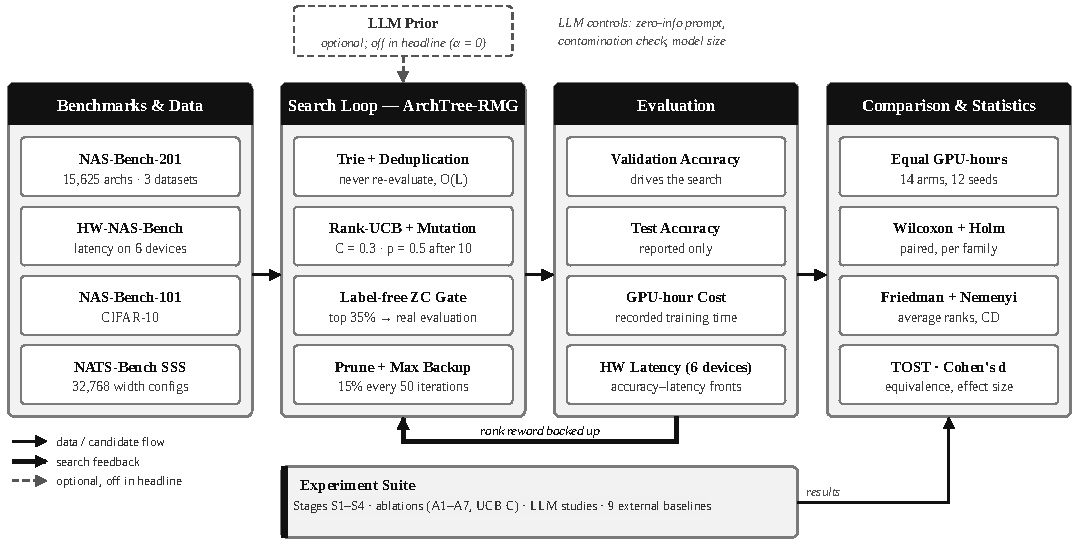
\includegraphics[width=0.92\textwidth]{figs/fig1_overview.pdf}
\caption{Overview of the study. Benchmarks give tabled accuracy, training time and latency; the \rmg{} loop generates, deduplicates and screens candidates; validation accuracy guides the search and test accuracy is only reported; methods get equal GPU-hours and are compared with paired and rank tests. The LLM prior (dashed) is off in the headline system.}
\label{fig:overview}
\end{figure*}

\textit{Naming.} The complete system is called \rmg: a prefix trie over architecture tokens (\algname) searched with \textbf{R}ank-normalised UCB, combined with tournament \textbf{M}utation, and filtered by a label-free zero-cost \textbf{G}ate. Its reduced forms follow the same convention: \algname-base is the original trie with raw-reward UCB ($C=\sqrt2$, mean backup) and no gate, and \algname-RM is \rmg{} without the gate. Where no suffix is given, \algname{} refers to \rmg. Figure~\ref{fig:overview} gives an overview of the study, and Figure~\ref{fig:loop} and Algorithm~\ref{alg:archtree} summarise the search loop described below. The results follow four development stages: \textbf{S1} = \algname-base; \textbf{S2} = S1 with a supervised zero-cost gate (weights fitted on 1,500 labelled architectures); \textbf{S3} = \algname-RM; \textbf{S4} = \rmg, the final system.

\subsection{Problem setting}\label{sec:setting}

A search space $\mathcal{A}$ is a finite set of architectures, each written as a token sequence $a=(o_1,\dots,o_L)$, where $o_\ell$ is drawn from a position-specific vocabulary $\mathcal{V}_\ell$. On NAS-Bench-201, $L=6$ edges each take one of five operations, so $|\mathcal{A}|=5^6=15{,}625$. Every architecture has a validation accuracy $A(a)$, a test accuracy $T(a)$ and a training cost $\tau(a)$ (GPU-seconds) recorded by the benchmark. A search proposes candidates one at a time; proposal $t$ either receives a \emph{real evaluation}, which reveals $A(a_t)$ and costs $\tau(a_t)$, or is skipped at negligible cost. Given a budget, the search returns the evaluated architecture with the highest validation accuracy, and we report its test accuracy. Searching on validation and reporting test accuracy follows the NAS-Bench-201 protocol \cite{dong2020} and prevents selection on the reported metric.

\subsection{Trie encoding and deduplication}

Every evaluated architecture is inserted into a prefix trie whose depth equals $L$; each internal node at depth $\ell$ represents all architectures that share the first $\ell$ tokens. Insertion and look-up take $O(L)$ time. Before a proposal is evaluated, the loop checks whether its leaf is already present; if so, the proposal is replaced by a random unvisited architecture. On NAS-Bench-101, tokens are five operations followed by 21 adjacency bits ($L=26$), and proposals that decode to an invalid or isomorphic cell are redirected in the same way, using the benchmark's graph hash. As a result, no architecture is trained twice, which holds by construction rather than as an empirical property.

\subsection{Rank-normalised UCB with mutation}

At a node $p$ the loop descends to the child
\begin{equation}
c^{*}=\arg\max_{c\,\in\,\mathcal{C}(p)}\left[\bar r(c)+C\sqrt{\frac{\ln N(p)}{n(c)}}\right],\label{eq:ucb}
\end{equation}
where $N(p)$ and $n(c)$ are visit counts, unvisited children are taken first, and ties are broken at random. The first design, \algname-base, used $\bar r(c)=A/100$ with $C=\sqrt{2}$. Because NAS-Bench-201 accuracies of good subtrees differ by only a few points, the exploration bonus (about 1--2.5) swamped differences of 0.01--0.05 in the value term and the descent became almost uniform. \rmg{} replaces the value with the percentile rank of the subtree's backed-up accuracy among all accuracies observed in the run,
\begin{equation}
r_t(a)=\frac{1}{t}\sum_{i=1}^{t}\mathbb{1}\left[A(a_i)\le A(a)\right]\in[0,1],\label{eq:rank}
\end{equation}
uses $C=0.3$ and backs up the maximum accuracy of each subtree. After ten real evaluations, each proposal is, with probability 0.5, replaced by a mutation of the best of five randomly drawn evaluated architectures (tournament selection as in RE \cite{real2019}), using the benchmark's own one-token mutation.

\subsection{Label-free zero-cost gate}\label{sec:gate}

Three proxies are computed on an untrained proxy-size network (32 channels, fixed initialisation): the SVD entropy $E$ of the centred final feature map \cite{roy2007}, SynFlow $S$ \cite{tanaka2020}, computed in double precision with batch normalisation in evaluation mode, and NASWOT $T$ \cite{mellor2021}, averaged over three fixed batches of 256 CIFAR-10 images. Each proxy is standardised with the mean and standard deviation of 1,500 randomly drawn \emph{unlabelled} architectures, and the gate score is their unweighted mean,
\begin{equation}
P(a)=\tfrac{1}{3}\left[z(E_a)+z(S_a)+z(T_a)\right].\label{eq:proxy}
\end{equation}
No accuracy label is used to build $P$. The first ten proposals always pass; afterwards proposal $a_t$ is evaluated only if
\begin{equation}
P(a_t)\ \ge\ q_{0.65}\{P(a_1),\dots,P(a_t)\},\label{eq:gate}
\end{equation}
that is, if it lies among the highest 35\% of the scores observed so far in the run. A rejected proposal only increments visit counts on its path. One proxy evaluation takes about 0.28\,s on a laptop GPU, roughly 1/6,500 of the mean NAS-Bench-201 CIFAR-10 training time. A supervised variant, with weights fitted to 1,500 labelled architectures, is kept for comparison and its labels are counted as cost.

\subsection{Optional LLM prior and pruning}

When enabled, an LLM receives the tokens fixed so far and the list of unvisited operations, and returns an integer score from 0 to 9 for each, under a strict JSON schema. Scores are converted to a distribution $p_{\mathrm{LLM}}$ and enter only the ordering of \emph{never-visited} children,
\begin{equation}
Q_{0}(c)=\alpha_t\,p_{\mathrm{LLM}}\big(o_c\mid \mathrm{prefix}(c)\big),\qquad \alpha_t=\alpha/\sqrt{t'},\label{eq:llm}
\end{equation}
where $t'$ is the iteration rescaled to a budget of 100; once $\alpha_t<0.02$ the prior is no longer queried. A zero-information prior reproduces the prior-off search exactly (24 of 24 seeds). In the headline system $\alpha=0$; the prior is studied separately in section~\ref{sec:llm}. Every 50 iterations the 15\% of internal nodes with the lowest backed-up accuracy, among those with at least two visits, are marked as pruned, never removing the last live child of a node.

\begin{figure*}[t]
\centering
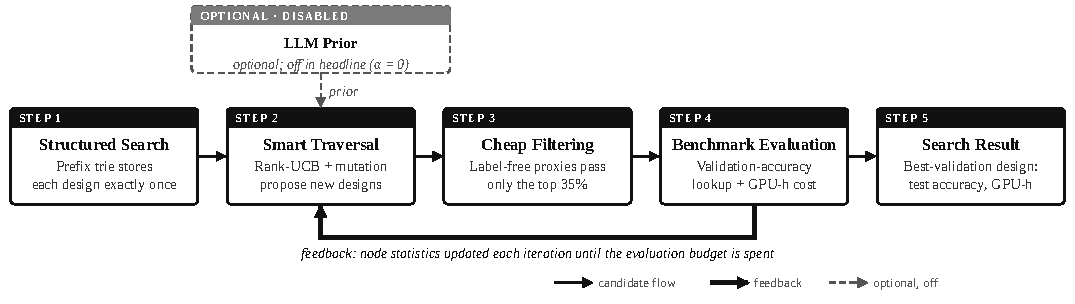
\includegraphics[width=\textwidth]{figs/fig2_pipeline.pdf}
\caption{The \rmg{} search loop in five steps. A compressed trie stores every evaluated design once (step 1); rank-normalised UCB descent and mutation propose a new design (step 2); the label-free proxy gate passes only the top 35\% (step 3); passing designs are looked up in the benchmark and charged their training time (step 4); statistics are fed back up the trie until the budget is spent, and the best-validation design is reported (step 5). The LLM prior (dashed) is off in the headline system; Algorithm~\ref{alg:archtree} gives the details.}
\label{fig:loop}
\end{figure*}

\begin{algorithm}[t]
\caption{\rmg{}: trie search with rank-normalised UCB, mutation and the label-free zero-cost gate}\label{alg:archtree}
\footnotesize
\begin{algorithmic}[1]
\Require benchmark $\mathcal{B}$, proposal budget $B$, gate pass rate $q=0.35$, warm-up $w=10$, $C=0.3$, mutation probability $p_m=0.5$, prior weight $\alpha$
\Ensure test accuracy, real evaluations and GPU-hours of the best-validation architecture
\State trie $\mathcal{T}\gets\emptyset$; history $\mathcal{H}\gets\emptyset$; scores $\mathcal{S}\gets\emptyset$; cost $G\gets 0$
\For{$t=1$ \textbf{to} $B$}
  \State $a\gets$ UCB descent of $\mathcal{T}$ (Eq.~\ref{eq:ucb}, values from Eq.~\ref{eq:rank}; unvisited children ordered by Eq.~\ref{eq:llm})
  \If{$|\mathcal{H}|\ge w$ \textbf{and} $u\sim U(0,1)<p_m$}
    \State $a\gets$ mutate(best of 5 random members of $\mathcal{H}$)
  \EndIf
  \If{$a\in\mathcal{T}$ \textbf{or} $a$ invalid} \State $a\gets$ random unevaluated architecture \EndIf
  \If{$t>w$}
    \State $\mathcal{S}\gets\mathcal{S}\cup\{P(a)\}$ \Comment{Eq.~\ref{eq:proxy}, no labels}
    \If{$P(a)<q_{1-q}(\mathcal{S})$} \State increment visit counts on the path of $a$; \textbf{continue} \EndIf
  \EndIf
  \State $A\gets$ validation accuracy of $a$; $G\gets G+\tau(a)$ \Comment{real evaluation}
  \State insert $a$ in $\mathcal{T}$; back up $\max$ accuracy and visits; $\mathcal{H}\gets\mathcal{H}\cup\{(a,A)\}$
  \If{$t \bmod 50=0$} \State prune 15\% lowest-value nodes ($\ge 2$ visits) \EndIf
\EndFor
\State $a^{*}\gets\arg\max_{(a,A)\in\mathcal{H}}A$
\State \Return $T(a^{*})$, $|\mathcal{H}|$, $G$
\end{algorithmic}
\end{algorithm}

\subsection{When should the gate penalise cost? A closed-form criterion}\label{sec:criterion}

Zero-cost proxies tend to prefer bigger networks, whose training is slower (section~\ref{sec:cost}). An obvious correction is to penalise predicted cost $D$ (here $\log(1+\#\text{params})$) in the gate score, $S_\lambda=z(P)-\lambda z(D)$. To decide in advance whether this helps, we replace accuracy $A$, proxy $P$ and predicted cost $D$ by their normal scores and treat them as jointly Gaussian with pairwise correlations $r_{PA}$, $r_{PD}$ and $r_{DA}$ (a Gaussian copula). The correlation between the penalised score and accuracy is then
\begin{equation}
\rho(S_\lambda,A)=\frac{r_{PA}-\lambda\,r_{DA}}{\sqrt{1+\lambda^{2}-2\lambda\,r_{PD}}},\label{eq:corr}
\end{equation}
and its slope at $\lambda=0$ is
\begin{equation}
\left.\frac{\partial\rho(S_\lambda,A)}{\partial\lambda}\right|_{\lambda=0}=r_{PA}\,r_{PD}-r_{DA}.\label{eq:slope}
\end{equation}
A small penalty improves the quality of what the gate admits only if $r_{DA}<r_{PA}r_{PD}$, i.e. only if accuracy is less coupled to cost than the proxy's own cost bias implies. If the slope is negative, the penalty can pay off only through the extra, cheaper evaluations it buys. To estimate that trade-off at a GPU-hour budget, we simulate gated random search in the fitted copula with the exact gate rule of Eq.~(\ref{eq:gate}). The derivation of Eq.~(\ref{eq:slope}) is given in Appendix~A. Every quantity comes from a sample of architectures drawn before the search starts, so the prediction precedes the result.

%% =====================================================================
\section{Experimental setup}\label{sec:setup}

\subsection{Benchmarks and data}\label{sec:data}

Table~\ref{tab:datastats} lists the benchmarks: NAS-Bench-201 \cite{dong2020} (six edges with five operations each), NAS-Bench-101 \cite{ying2019} (cell graphs with up to seven nodes and nine edges), the size space of NATS-Bench \cite{dong2022} (five layer widths from $\{8,16,\dots,64\}$) and HW-NAS-Bench \cite{li2021hw}, which adds the latency of every NAS-Bench-201 cell on six devices (edge GPU and TPU, Raspberry Pi 4, Pixel 3, Eyeriss, FPGA). Datasets are CIFAR-10/100 (C10/C100) \cite{krizhevsky2009} and ImageNet16-120 (IN16) \cite{chrabaszcz2017}. Accuracies and training times are read from tables and nothing is trained during search; a search is charged the recorded training time of each architecture it evaluates. Tabular benchmarks are used deliberately: they make thousands of complete, seed-paired searches affordable, they remove training noise from the comparison of search strategies, and they let every claim be checked against the exhaustive ground truth of the space \cite{ying2019,dong2020,yang2020}. The three spaces were chosen to differ in the property that matters most for a proxy gate. NAS-Bench-201 is a small cell space and the main test bed. NAS-Bench-101 is a much larger cell space with variable graph topology, on which proxies are known to be weaker \cite{krishnakumar2022}, so it tests transfer. The size space of NATS-Bench fixes the cell and varies only channel widths, so accuracy and cost are both driven by network width; it is the natural stress test for the claim that proxies detect cost (section~\ref{sec:cost}).


\textit{How the data are kept.} The raw benchmark files (roughly 6.5\,GB in total) are turned once into compact derived caches, the only files the experiments read (Table S42). Each record is keyed by a canonical code of the architecture (base 5 over the NAS-Bench-201 edges, base 8 over the NATS-Bench widths, the official module hash for NAS-Bench-101) and holds a validation accuracy for search, a test accuracy for reporting and a training time for cost: 200-epoch values averaged over training seeds for NAS-Bench-201, the 90-epoch schedule for NATS-Bench SSS and the mean of three 108-epoch repeats for NAS-Bench-101. The NAS-Bench-101 cache is read from the TFRecord file with a reimplementation of the official graph pruning and hashing, and the build fails unless all 423,624 module hashes are reproduced. HW-NAS-Bench latencies are aligned to NAS-Bench-201 indices, and the exact Pareto front of each device is precomputed. Raw proxy components are stored once per architecture (70,765 entries), so every search re-uses identical proxy values. The benchmark files and main caches are fixed by SHA-256 checksums (Table S41), and every search writes one result row per run.


\begin{figure*}[t]
\centering
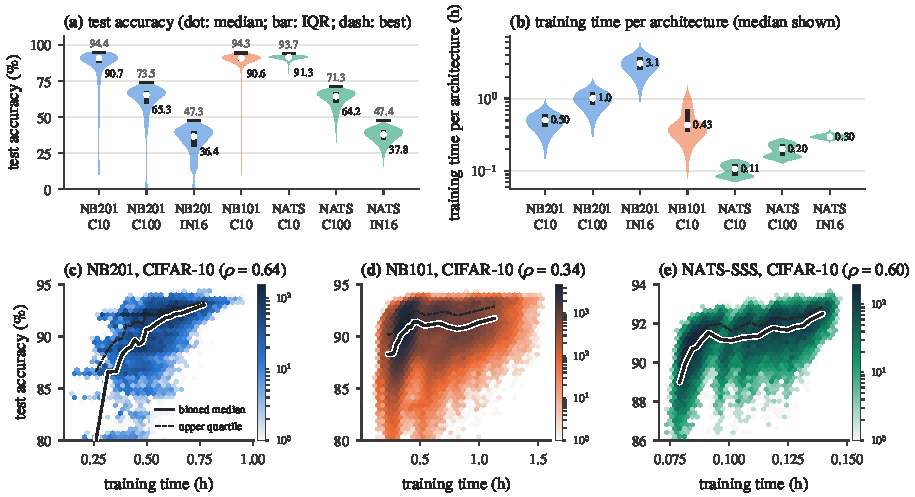
\includegraphics[width=\textwidth]{figs/fig3_datasets.pdf}
\caption{The three search spaces as data. (a) Test-accuracy distribution of every architecture (violin), with inter-quartile range (bar), median (dot) and best architecture (dash). (b) Distribution of the recorded training time of one architecture (log scale). (c)--(e) Test accuracy against training time on CIFAR-10 (hexagonal bins, log counts; the panels show the 89\%, 98\% and almost 100\% of each space above the plotted accuracy floor). In every space, more expensive architectures tend to be more accurate, but much less steeply in NAS-Bench-101, and NATS-SSS forms separate bands, one for each width of the most expensive layer.}
\label{fig:data}
\end{figure*}

\begin{table*}[t]
\caption{Statistics of the full search spaces (all architectures; accuracies in \%, training time per architecture in GPU-hours).}\label{tab:datastats}
\centering\footnotesize
\setlength{\tabcolsep}{4.2pt}
\begin{tabular}{@{}llrrcccccc@{}}
\toprule
Benchmark & Data & $|\mathcal{A}|$ & Epochs & Test mean $\pm$ s.d. & Best & 99th pct. & $\bar\tau$ [min, max] (h) & CV($\tau$) & $\rho$(valid, test) / $\rho$(test, $\tau$)\\
\midrule
NB201 & C10 & 15,625 & 200 & 87.06 $\pm$ 12.94 & 94.37 & 93.78 & 0.51 [0.15, 0.96] & 0.26 & 0.983 / 0.64\\
NB201 & C100 & 15,625 & 200 & 61.39 $\pm$ 12.17 & 73.51 & 71.15 & 1.02 [0.30, 1.92] & 0.26 & 0.993 / 0.65\\
NB201 & IN16 & 15,625 & 200 & 33.57 $\pm$ 9.51 & 47.31 & 45.40 & 3.08 [0.91, 5.83] & 0.26 & 0.994 / 0.62\\
NB101 & C10 & 423,624 & 108 & 89.68 $\pm$ 5.80 & 94.32 & 93.51 & 0.54 [0.08, 1.53] & 0.48 & 0.995 / 0.34\\
NATS-SSS & C10 & 32,768 & 90 & 91.09 $\pm$ 1.27 & 93.65 & 93.05 & 0.11 [0.07, 0.15] & 0.18 & 0.963 / 0.60\\
NATS-SSS & C100 & 32,768 & 90 & 62.64 $\pm$ 5.63 & 71.34 & 69.76 & 0.20 [0.13, 0.28] & 0.19 & 0.986 / 0.27\\
NATS-SSS & IN16 & 32,768 & 90 & 37.09 $\pm$ 4.75 & 47.40 & 44.97 & 0.30 [0.24, 0.38] & 0.06 & 0.979 / 0.51\\
\bottomrule
\end{tabular}
\tablenotes{CV: coefficient of variation of training time. $\rho$: Spearman correlation over the whole space. The best test accuracy is not attainable by a validation-based search when validation and test rankings disagree.}
\end{table*}


Figure~\ref{fig:data} and Table~\ref{tab:datastats} describe the spaces as data. Three properties shape the experiments. First, the spaces are top-heavy: the gap between the best architecture and the 99th percentile is only 0.6 points on NAS-Bench-201 CIFAR-10 and NATS-Bench SSS CIFAR-10, so good methods differ by tenths of a point. Second, a long tail of poor architectures exists on NAS-Bench-201 (341 architectures below 20\% on CIFAR-10; exactly the cells disconnected by \texttt{none} operations), which a cheap filter can remove. Third, accuracy and training time are positively correlated in every space ($\rho$ = 0.27--0.65), so a filter that prefers accurate networks will also prefer expensive ones; hence cost is measured in GPU-hours.

\subsection{Baselines and arms}

Nine external baselines run on all three NAS-Bench-201 datasets with the same seeds: random search \cite{li2020random}; RE \cite{real2019}; RE with a zero-cost warm-up (population seeded with the best of 1,000 proxy-scored architectures \cite{abdelfattah2021}); local search (LS) \cite{white2021ls}; ENAS-style policy search \cite{pham2018}; MCTS-style search \cite{wang2020alphax}; ZiCo-style proxy-guided sampling \cite{li2023zico}; an RZ-style zero-cost mutation walk; and an LLM generator (LLM-NAS, \texttt{gpt-oss-20b} \cite{openai2025gptoss}, eight architectures per call, best-so-far context) in the style of \cite{zheng2023genius}. The re-implemented baselines carry the suffix ``-style''. They were chosen to cover the four families that dominate sample-based NAS (random, evolutionary, local, policy/tree search), the two existing ways of using zero-cost proxies (warm-up and proxy-guided sampling) and LLM generation. Internal arms include \algname{} without the gate, with a parameter-count gate, with a supervised gate and with cost-penalised gates ($\lambda=0.25$ and 1), a flat UCB over positions (with or without deduplication), and random and NSGA-II-style \cite{deb2002} search for the hardware study. Every proposer was also run with every gate (none, \#params, supervised, label-free), which separates the contribution of the gate from that of the proposer.

\subsection{Protocol and cost accounting}

NAS-Bench-201 budgets are 25, 50, 100 and 200 proposals, which spans the range used in the literature for this space (about 0.2--1.3\% of it); NAS-Bench-101 budgets are 50, 100, 200 and 400 because the space is 27 times larger. Every configuration is run on 12 seeds, which, given the seed-to-seed spread (typically 0.1--0.8 points), resolves paired differences of a few tenths of a point; the base$\to$RMG design changes were re-tested on 12 further held-out seeds that were never used for any design decision. In the \emph{equal-GPU-hour} protocol each arm is run once with a large proposal budget and its evaluation history is cut at
\begin{equation}
H_k=k\,\bar\tau,\qquad \sum_{a\in\mathcal{E}}\tau(a)\le H_k,\qquad k\in\{25,50,100\},\label{eq:egh}
\end{equation}
where $\bar\tau$ is the average time needed to train a single architecture of that benchmark and dataset (Table~\ref{tab:datastats}) and $\mathcal{E}$ is the set of evaluated architectures. Because no arm plans with the budget, truncation is equivalent to running with budget $H_k$. Fourteen arms on NAS-Bench-201 and NATS-Bench SSS and ten on NAS-Bench-101, with 12 seeds, give 1,128 runs. Proxy time is charged as well; at 0.28\,s per scored proposal it adds at most 0.05\% to a NAS-Bench-201 budget and of the order of 0.2\% on NATS-Bench SSS, whose networks train fastest.

\begin{table}[t]
\caption{Experimental campaign: stages, purpose and number of complete search runs.}\label{tab:campaign}
\centering\footnotesize
\setlength{\tabcolsep}{2.5pt}
\begin{tabular}{@{}>{\raggedright\arraybackslash}p{0.33\columnwidth}>{\raggedright\arraybackslash}p{0.47\columnwidth}>{\raggedleft\arraybackslash}p{0.14\columnwidth}@{}}
\toprule
Stage & Question answered & Runs\\
\midrule
Baselines & reference performance (9 methods) & 1,296\\
S1 \algname-base & does a deduplicating tree search work? & 144\\
S2 + supervised gate & how much does a proxy gate save? & 144\\
S4 \rmg{} & headline system & 144\\
Proposer $\times$ gate grid & is the gate portable? (6 proposers $\times$ 4 gates) & 3,456\\
Held-out design ablation & which design change matters? (new seeds) & 720\\
Trie vs flat bandit (A7) & hierarchy or deduplication? & 432\\
Toggle ablations (A1--A6) & LLM, gate, inheritance, $\alpha$, pruning, budget & 792\\
UCB sensitivity & $C$ and backup rule & 1,008\\
Proxy subsets & which proxies in the gate? & 612\\
LLM studies & speed, $\alpha$ sweep, model size & 973\\
NAS-Bench-101 & transfer to a larger space & 576\\
Equal GPU-hours & fair-cost comparison, 3 benchmarks & 1,128\\
Hardware (HW-NAS-Bench) & accuracy--latency search & 864\\
\midrule
Total & & 12,289\\
\bottomrule
\end{tabular}
\tablenotes{Counts are complete search runs recorded in the result files. S3 (\algname-RM) is part of the proposer $\times$ gate grid. The LLM knowledge probe adds 672 queries.}
\end{table}

Table~\ref{tab:campaign} lists the stages of the work: 12,289 complete, logged searches with fixed seeds, the sole source of every reported result.

\subsection{Statistics}

Comparisons are paired by seed. We use two-sided Wilcoxon signed-rank tests \cite{wilcoxon1945} with Holm correction \cite{holm1979} within each comparison family and report a result as a win or loss only if $p_{\mathrm{Holm}}<0.05$. Across methods, we use the Friedman test with blocks (dataset, budget, seed) and the Nemenyi critical difference (CD) \cite{demsar2006}. Because a non-significant difference does not show that two methods are equal, two one-sided tests (TOST) \cite{schuirmann1987} with margins of $\pm$0.5 and $\pm$0.25 points are reported as well, along with the probability that \algname{} beats a method, with stratified-bootstrap 95\% confidence intervals \cite{agarwal2021}. Where an LLM-guided trajectory is identical for all seeds, paired differences that do not vary between seeds are not tested.

\subsection{Implementation}

The code is in Python 3.10 with PyTorch 2.5.1; proxies run on an NVIDIA RTX 2050 (4 GB). The LLM is \texttt{gpt-oss-20b} \cite{openai2025gptoss} served by Groq, with answers cached by prompt; no LLM-prior run used a fallback answer. Runs are deterministic (all checks: Table S40). Table~\ref{tab:rationale} lists the settings, all frozen before the final runs and shared by every reported run.


\subsection{Why these settings}\label{sec:rationale}

Each setting in Table~\ref{tab:rationale} is either justified by a measurement on the full space or shown not to matter (Figure~\ref{fig:design}).

\textit{Pass rate.} Ranking all 15,625 NAS-Bench-201 architectures by the label-free score and admitting the top fraction $q$ gives the operating curve of Figure~\ref{fig:design}(a). The smallest $q$ that keeps every architecture of the top 5\% (by validation accuracy) is 34\%, 34\% and 29\% on the three datasets, and at $q=0.35$ the gate keeps 100\% of both the top 1\% and the top 5\% on all three; on NATS-Bench SSS it keeps 98.5--100\% of the top 1\%. A tighter gate starts to lose good architectures (at $q=0.2$ only 80\% of the CIFAR-10 top 5\% survive), while a looser gate only adds cost. The search applies the same quantile to the scores seen so far, which approximates this whole-space threshold once enough proposals have been scored.

\textit{Cost of what passes.} Figure~\ref{fig:design}(b) shows the price of this choice. On NAS-Bench-201 the admitted 35\% train 1.22 times longer than an average architecture, whereas the truly best 35\% train 1.16--1.18 times longer; the proxy therefore over-pays by only 3--5\%. On NATS-Bench SSS (full space) the architectures that pass are cheaper still than the true top set (1.02--1.05 against 1.03--1.12).

\textit{Proxy composition.} The gate averages $E$, $S$ and $T$ and leaves out the size term $C$ of the proxy cache. Among all 15 subsets of the four components used as gates (Figure~\ref{fig:design}(d)), the three-proxy set is among the best-ranked ($\tau$ = 0.66, 0.71 and 0.62) and keeps 93--100\% of the top 5\%, whereas adding the size term lowers that recall on CIFAR-10 to 80\%; no subset is significantly better than the four-component set (2 of 48 tests against it differ, both because SVD entropy alone is worse). Across the 15 subsets, a subset's rank correlation hardly predicts the accuracy of the search that uses it (Spearman 0.02, 0.15 and 0.54), whereas its recall of the top 5\% does better on CIFAR-100 (0.77, $p<0.001$): a gate must keep the best architectures, not rank the whole space. Leaving out an explicit size term is also what the criterion of section~\ref{sec:criterion} recommends.

\textit{UCB, warm-up and pruning.} Of 14 combinations of $C\in\{0.1,0.2,0.3,0.5,1,1.414,2\}$ with mean or max backup (Figure~\ref{fig:design}(c)), $C=0.3$ with max backup has the highest mean accuracy, the others lying 0.02--0.31 points below, but none of the 78 differences is significant. Ten unconditional proposals give the running quantile and the tournament a minimum sample, and pruning thresholds from 0 to 35\% change accuracy by less than the seed-to-seed spread.


\begin{table}[t]
\caption{Settings of \rmg{} (identical in all reported runs) and the evidence for each.}\label{tab:rationale}
\centering\footnotesize
\setlength{\tabcolsep}{2.5pt}
\begin{tabular}{@{}>{\raggedright\arraybackslash}p{0.25\columnwidth}>{\raggedright\arraybackslash}p{0.71\columnwidth}@{}}
\toprule
Choice & Evidence (section)\\
\midrule
Trie & no repeated evaluation by construction; flat bandit wastes 73--74\% (\ref{sec:ablation})\\
Rank reward & raw reward gives near-uniform descent; the base design is 0.63\,pt worse on held-out seeds (\ref{sec:ablation})\\
Mutation $p_m=0.5$ & carries most of the accuracy; mutation-only is level with \rmg{} (\ref{sec:ablation})\\
$C=0.3$, max backup & best of 14 settings; 0/78 significant differences (Fig.~\ref{fig:design}c)\\
Gate $q=0.35$ & smallest round rate keeping all top-5\% NB201 architectures (Fig.~\ref{fig:design}a)\\
$E+S+T$, no labels & $\tau$ within 0.04 of the supervised ensemble; size term lowers recall (Fig.~\ref{fig:design}d)\\
No cost penalty & criterion slope $<0$ on 7/7 pairs; penalty loses 16/21 cells (\ref{sec:cost})\\
LLM prior off & faster start only; no final-accuracy gain (\ref{sec:llm})\\
Pruning 15\% & 0--35\% indistinguishable (\ref{sec:ablation})\\
Warm-up 10, tournament 5 & minimum sample for the quantile and the tournament\\
z-stats from 1,500 archs & unlabelled sample; weights $E=S=T=\tfrac13$\\
Seeds & 12 main + 12 held-out for design checks\\
\bottomrule
\end{tabular}
\end{table}

\begin{figure*}[t]
\centering
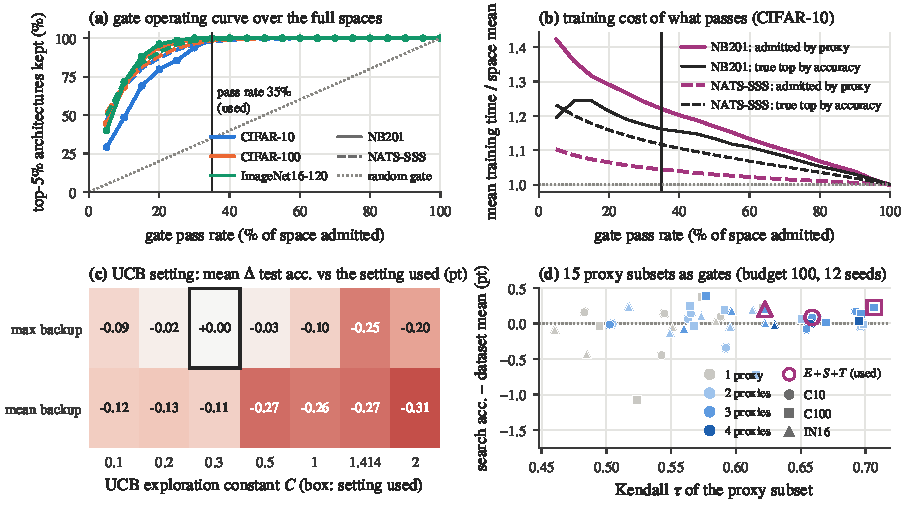
\includegraphics[width=\textwidth]{figs/fig5_design_choices.pdf}
\caption{Evidence for the settings of \rmg{}. (a) Share of the top-5\% architectures (by validation accuracy) that a static label-free gate keeps when it admits a fraction $q$ of the whole space; the vertical line marks $q=0.35$ and the dotted diagonal is a random gate. (b) Mean training time of what the gate admits, divided by the mean over the space (red), compared with the truly best fraction $q$ (black). (c) Mean change in test accuracy of each UCB setting relative to the one used, averaged over three datasets and two budgets (12 seeds each). (d) Each of the 15 proxy subsets acting as gate: rank correlation against search accuracy at budget 100, relative to the mean over subsets; circles mark the subset used.}
\label{fig:design}
\end{figure*}

\begin{table*}[t]
\caption{NAS-Bench-201, budget 200 proposals: test accuracy (\%) of the best-validation architecture, mean $\pm$ standard deviation over 12 seeds, with real evaluations and GPU-hours (C10 / C100 / IN16). Best accuracy per column in bold; S1--S3: means only.}\label{tab:main}
\centering\footnotesize
\begin{tabular}{@{}lccccc@{}}
\toprule
Method & Real evals & GPU-h & CIFAR-10 & CIFAR-100 & ImageNet16-120\\
\midrule
Random search \cite{li2020random} & 200 & 102 / 204 / 619 & 93.92 $\pm$ 0.21 & 71.92 $\pm$ 0.81 & 45.47 $\pm$ 0.80\\
MCTS-style \cite{wang2020alphax} & 200 & 103 / 207 / 630 & 93.89 $\pm$ 0.20 & 71.94 $\pm$ 0.87 & 45.44 $\pm$ 0.65\\
ENAS-style \cite{pham2018} & 200 & 115 / 236 / 717 & 94.09 $\pm$ 0.26 & 72.59 $\pm$ 0.81 & 46.16 $\pm$ 0.36\\
LLM-NAS (\texttt{gpt-oss-20b}) & 200 & 140 / 274 / 825 & 94.28 $\pm$ 0.08 & 72.14 $\pm$ 0.43 & 45.37 $\pm$ 0.36\\
ZiCo-style \cite{li2023zico} & 200 + proxy & 138 / 275 / 835 & 94.29 $\pm$ 0.12 & 72.97 $\pm$ 0.43 & 46.28 $\pm$ 0.57\\
RZ-style ZC walk & 200 + proxy & 149 / 298 / 906 & 94.33 $\pm$ 0.07 & 73.39 $\pm$ 0.19 & 46.32 $\pm$ 0.18\\
RE \cite{real2019} & 200 & 121 / 258 / 782 & 94.31 $\pm$ 0.13 & 73.37 $\pm$ 0.21 & 46.48 $\pm$ 0.17\\
RE + ZC warm-up \cite{abdelfattah2021} & 200 + proxy & 125 / 263 / 820 & 94.28 $\pm$ 0.19 & 73.36 $\pm$ 0.23 & 46.34 $\pm$ 0.36\\
Local search \cite{white2021ls} & 200 & 124 / 254 / 777 & \textbf{94.37 $\pm$ 0.00} & \textbf{73.51 $\pm$ 0.00} & \textbf{46.52 $\pm$ 0.29}\\
\midrule
S1: \algname-base (trie + UCB) & 200 & 112 / 236 / 690 & 94.11 & 73.12 & 46.25\\
S2: S1 + supervised gate & 62--65 & 39 / 83 / 252 & 94.17 & 72.45 & 46.39\\
S3: \algname-RM (no gate) & 200 & 117 / 243 / 742 & 94.12 & 72.97 & 46.39\\
\algname-RM + supervised gate (1,500 labels) & 76--81 & 54 / 112 / 348 & 94.26 & 73.27 & 46.43\\
S4: \rmg{} (ours) & 81--83 & 55 / 115 / 351 & 94.28 $\pm$ 0.13 & 73.40 $\pm$ 0.20 & 46.41 $\pm$ 0.18\\
\midrule
Best architecture in the space (by validation) & -- & -- & 94.37 & 73.51 & 46.20\\
\bottomrule
\end{tabular}
\tablenotes{``+ proxy'': every proposal is also proxy-scored. GPU-h are recorded 200-epoch training times of the evaluated architectures; the S2 GPU-h is low because its supervised gate admits fewer proposals. On ImageNet16-120 several methods exceed the best-validation architecture in test accuracy because validation and test rankings differ slightly.}
\end{table*}

%% =====================================================================
\section{Results}\label{sec:results}

\begin{figure*}[t]
\centering
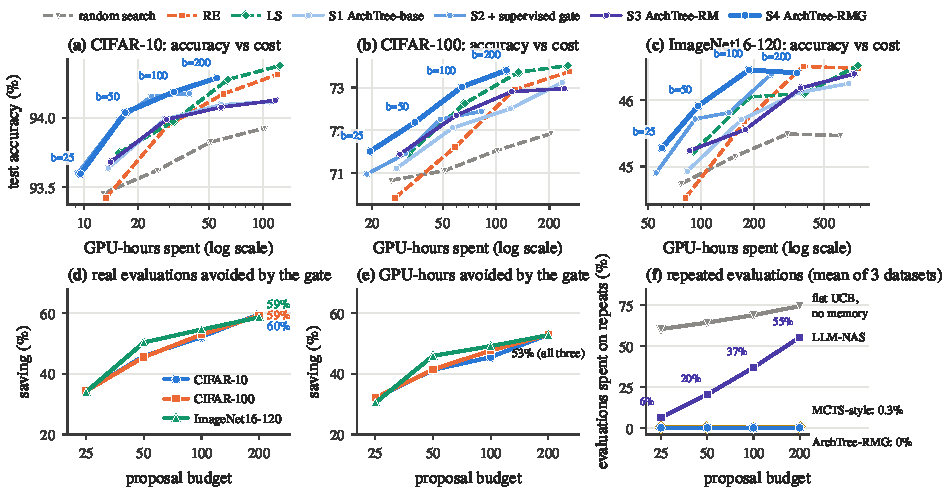
\includegraphics[width=\textwidth]{figs/fig6_stages.pdf}
\caption{Stage-wise development on NAS-Bench-201 (12 seeds). (a)--(c) Test accuracy against GPU-hours spent, one marker per proposal budget (25, 50, 100, 200; labelled for S4); further up and to the left is better. (d), (e) Real evaluations and GPU-hours that the label-free gate saves when added to \algname-RM at the same proposal budget. (f) Share of real evaluations spent on architectures that had already been trained. Stages: S1 = \algname-base (trie + raw-reward UCB); S2 = S1 + supervised gate; S3 = \algname-RM (rank UCB + mutation, no gate); S4 = \rmg{} (S3 + label-free gate).}
\label{fig:stages}
\end{figure*}

\subsection{Stage-wise development}\label{sec:stages}

Figure~\ref{fig:stages}(a)--(c) and the lower block of Table~\ref{tab:main} follow the system through its four stages. S1, a deduplicating trie searched by UCB with raw reward and mean backup, already beats random search (94.11 against 93.92 on CIFAR-10 at budget 200) but remains behind RE and LS. S2 adds a supervised zero-cost gate to S1: it cuts GPU-hours by 64--65\%, but on CIFAR-100 its accuracy drops by 0.67 points (not tested), plausibly because a near-uniform descent of the tree, given fewer evaluations, reaches fewer good regions. S3 replaces the raw reward by the rank reward and adds tournament mutation; it matches S1 on CIFAR-10, is 0.15 points lower on CIFAR-100 and 0.14 points higher on ImageNet16-120, but, without a gate, spends as much as RE. S4 adds the label-free gate to S3 and combines the two benefits: 94.28, 73.40 and 46.41 while evaluating 81--83 architectures and spending 47\% of the GPU-hours of S3. In the accuracy--cost plane S4 forms the upper-left edge of every panel (S2 touches it once, on CIFAR-10 at about 24 GPU-hours); ungated RE and LS reach final accuracies within $-0.03$ to $+0.11$ points of S4 at 2.2--2.3 times its GPU-hours, and RE with the same gate at 1.2--1.3 times.

The gate's savings grow with budget (Figure~\ref{fig:stages}(d), (e)), mainly because the ten unconditional warm-up proposals form a shrinking share of the budget, while the pass rate after warm-up stays near 35\%. At a budget of 200 it removes 59--60\% of real evaluations and 53\% of GPU-hours on all three datasets, while test accuracy changes by $+0.16$, $+0.43$ and $+0.02$ points. GPU-hour savings are about six points below the evaluation savings since the architectures that pass the gate are larger and slower to train, as anticipated by Figure~\ref{fig:design}(b). Figure~\ref{fig:stages}(f) shows the other source of waste: a flat bandit without memory spends 60--75\% of its evaluations on repeats and an LLM generator 6\% at budget 25 rising to 55\% at budget 200, whereas the trie spends none.

\begin{figure*}[t]
\centering
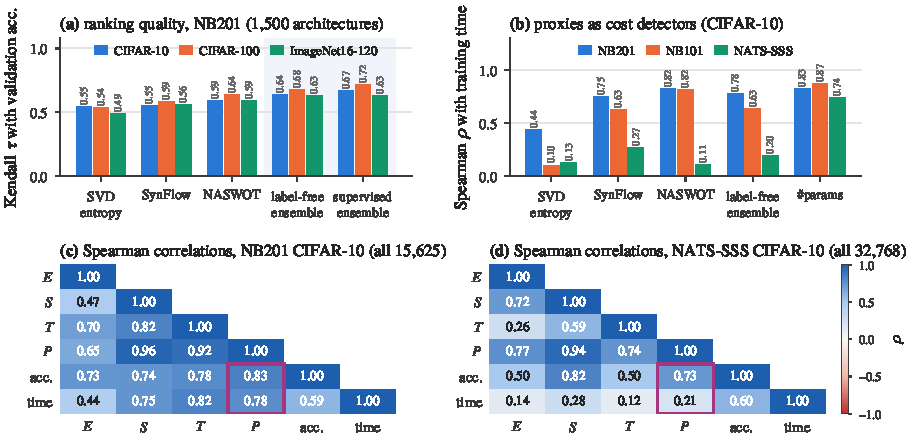
\includegraphics[width=\textwidth]{figs/fig4_proxies.pdf}
\caption{Zero-cost proxies. (a) Kendall $\tau$ between each proxy and validation accuracy (1,500 NAS-Bench-201 architectures); the label-free ensemble uses no labels and almost matches the supervised one. (b) Spearman $\rho$ between proxy score and recorded training time in the cell spaces NB201 (all 15,625 architectures) and NB101 (2,000), and the width space NATS-SSS (2,000). (c), (d) Spearman correlations between the three proxies, the label-free score $P$, validation accuracy and training time over the complete spaces; the boxed cells show that $P$ is as strongly related to training time as to accuracy on NB201, but only to accuracy on NATS-SSS.}
\label{fig:proxies}
\end{figure*}

\subsection{Proxy quality without labels}

Figure~\ref{fig:proxies}(a) shows the Kendall rank correlation $\tau$ \cite{kendall1938} of each proxy with validation accuracy on 1,500 NAS-Bench-201 architectures. Single proxies reach $\tau$ = 0.49--0.64. The label-free ensemble reaches 0.64, 0.68 and 0.63 on the three datasets (0.64, 0.67 and 0.64 over all 15,625 architectures), close to the supervised ensemble (0.67, 0.72, 0.63) that consumes 1,500 labels, and a search with the supervised gate reaches almost the same accuracy as the label-free one (Table~\ref{tab:main}). The components are complementary (Figure~\ref{fig:proxies}(c)): SVD entropy correlates only 0.47 with SynFlow, and averaging lifts the correlation with accuracy to 0.83, above any single proxy (0.73--0.78). On samples of 2,000 random architectures, proxy quality is lower on NAS-Bench-101 ($\tau$ = 0.33 label-free, 0.50 supervised) and intermediate on NATS-Bench SSS (0.53--0.63).

\begin{figure*}[t]
\centering
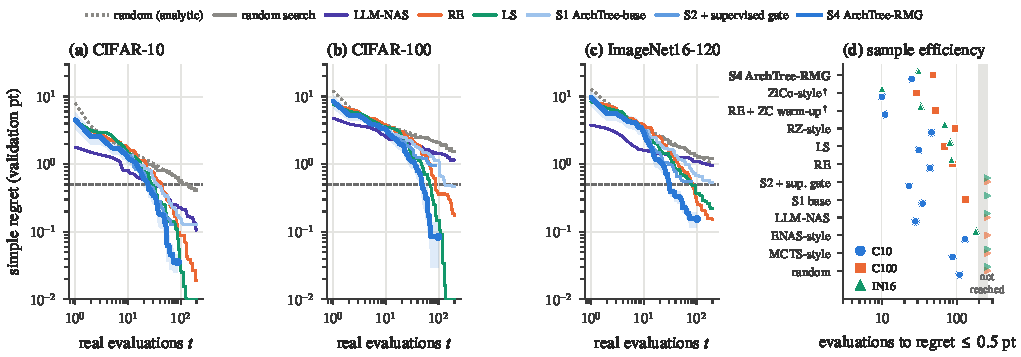
\includegraphics[width=\textwidth]{figs/fig7_convergence.pdf}
\caption{Convergence on NAS-Bench-201 at a budget of 200 proposals: simple regret (best validation accuracy in the space minus the best found so far, mean of 12 seeds; band: $\pm$1 standard error for S4) against the number of real evaluations. Gated stages stop earlier on the horizontal axis because they evaluate fewer proposals; the dotted line is the exact expectation for uniform random search without replacement and the dashed line marks 0.5 points. (d) Number of real evaluations at which the mean regret first reaches 0.5 points ($\triangleright$: not reached within 200); $^\dagger$these methods pick their first evaluations from 1,000 proxy-scored candidates. S1 = \algname-base, S2 = S1 + supervised gate, S4 = \rmg.}
\label{fig:conv}
\end{figure*}

\subsection{Convergence}

Figure~\ref{fig:conv} plots simple regret against real evaluations (all methods: Figure S3). Random search follows its analytic expectation, LLM-NAS starts lowest but flattens as it repeats itself, and S4 falls fastest of the \algname{} stages. At its last real evaluation (at most 88, 98 and 102 on the three datasets) S4 is within 0.04, 0.08 and 0.15 validation points of the best architecture of the space, against 0.41, 1.55 and 1.22 for random search after 200 evaluations and 0.02, 0.17 and 0.15 for RE. In Figure~\ref{fig:conv}(d), \rmg{} gets to within 0.5 points of the optimum in 25, 48 and 31 real evaluations, against 44, 88 and 85 for RE and 31, 69 and 81 for LS, while random search, MCTS-style search and LLM-NAS reach this level only on CIFAR-10, if at all. Only the two methods that pre-screen 1,000 proxy-scored candidates (ZiCo-style, and RE with ZC warm-up on CIFAR-10) get there sooner.

\subsection{Comparison with baselines at a fixed proposal budget}

Table~\ref{tab:main} reports test accuracy at a budget of 200, together with real evaluations and GPU-hours. Baselines evaluate all 200 proposals; \algname{} evaluates about 81--83 of them and uses 44--46\% of the GPU-hours of ungated RE. In the scorecard (Figure~\ref{fig:scorecard}), local search and RE with ZC warm-up are best on accuracy and rank, \rmg{} leads on cost with 41\% of the evaluations and 37--57\% of the GPU-hours of the baselines, and only the proxy-screening methods reach low regret with fewer real evaluations. The 108 paired tests (nine baselines, three datasets, four budgets) break down as follows. With Holm correction within each baseline, \algname{} records 20 wins, 88 ties and no losses; the wins split as random search 7, MCTS-style 6, ENAS-style and LLM-NAS 3 each, ZiCo-style 1. Without correction there are 32 wins and 6 losses, three of them against RE with zero-cost warm-up at budget 25 (93.91, 72.00, 46.11 against 93.60, 71.51, 45.28), where the ten unfiltered warm-up proposals are a weakness; TOST shows equivalence within $\pm$0.5 points in 27 of the 108 cells. In the Friedman ranking at a fixed proposal budget (10 methods, 144 blocks, CD = 1.13), \algname{} ranks 4.41, behind RE with zero-cost warm-up (3.67) and local search (3.90) yet inside the CD of both, with roughly 40\% of their evaluations. Table~\ref{tab:published} adds published NAS-Bench-201 results for context.

\begin{table}[!t]
\caption{Published NAS-Bench-201 results (test accuracy, \%, mean $\pm$ s.d. as reported) and \rmg{} at a budget of 200 proposals. Protocols differ, so this is context, not a paired comparison.}\label{tab:published}
\centering\scriptsize
\setlength{\tabcolsep}{1.4pt}
\begin{tabular}{@{}lclccc@{}}
\toprule
Method & Type & Budget & CIFAR-10 & CIFAR-100 & IN16-120\\
\midrule
Random search \cite{dong2020} & S & 12,000\,s$^a$ & 93.70$\pm$0.36 & 71.04$\pm$1.07 & 44.57$\pm$1.25\\
REA \cite{dong2020} & S & 12,000\,s$^a$ & 93.92$\pm$0.30 & 71.84$\pm$0.99 & 45.54$\pm$1.03\\
BOHB \cite{dong2020} & S & 12,000\,s$^a$ & 93.61$\pm$0.52 & 70.85$\pm$1.28 & 44.42$\pm$1.49\\
DARTS-V2 \cite{dong2020} & W & 35,782\,s & 54.30$\pm$0.00 & 15.61$\pm$0.00 & 16.32$\pm$0.00\\
GDAS \cite{dong2020} & W & 31,610\,s & 93.61$\pm$0.09 & 70.70$\pm$0.30 & 41.71$\pm$0.98\\
DrNAS$^b$ \cite{chen2021drnas} & W & -- & 94.36$\pm$0.00 & 73.51$\pm$0.00 & 46.34$\pm$0.00\\
NASWOT \cite{mellor2021} & T & 306\,s & 92.96$\pm$0.81 & 69.98$\pm$1.22 & 44.44$\pm$2.10\\
TE-NAS \cite{chen2021tenas} & T & 1,558\,s & 93.9$\pm$0.47 & 71.24$\pm$0.56 & 42.38$\pm$0.46\\
GENIUS$^b$ \cite{zheng2023genius} & L & 10 arch. & 93.79$\pm$0.09 & 70.91$\pm$0.72 & 44.96$\pm$1.02\\
\midrule
\rmg{}$^b$ (ours) & S+T & 81--83 arch. & 94.28$\pm$0.13 & 73.40$\pm$0.20 & 46.41$\pm$0.18\\
Optimal \cite{dong2020} & -- & -- & 94.37 & 73.51 & 47.31\\
\bottomrule
\end{tabular}
\tablenotes{S: sample-based; W: weight-sharing; T: training-free; L: LLM-based. Budget: GPU search time or architectures trained per run; $^a$simulated. $^b$Searched on each dataset; the others search on CIFAR-10 and transfer.}
\end{table}


\begin{figure*}[t]
\centering
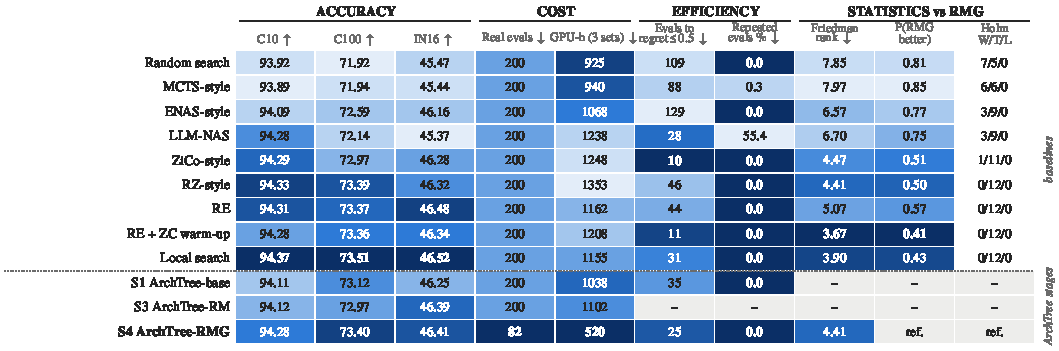
\includegraphics[width=\textwidth]{figs/fig17_scorecard.pdf}
\caption{Method scorecard on NAS-Bench-201 at a budget of 200 proposals (12 seeds). Each cell shows the raw value; shading ranks the methods within each column (darker = better, best in bold; grey = not available). Accuracy is the test accuracy of the best-validation architecture; GPU-h is summed over the three datasets; evaluations to regret $\leq$0.5 and repeated evaluations are for CIFAR-10 and the mean of the three datasets, respectively. Statistics compare each baseline with \rmg{} over 12 dataset--budget cells: Friedman average rank (10 methods, 144 blocks, CD = 1.13), bootstrap probability that \rmg{} wins a paired run (darker = stronger rival) and Holm-corrected wins/ties/losses of \rmg. S1, S3, S4: development stages (section~\ref{sec:method}).}
\label{fig:scorecard}
\end{figure*}

\begin{figure*}[t]
\centering
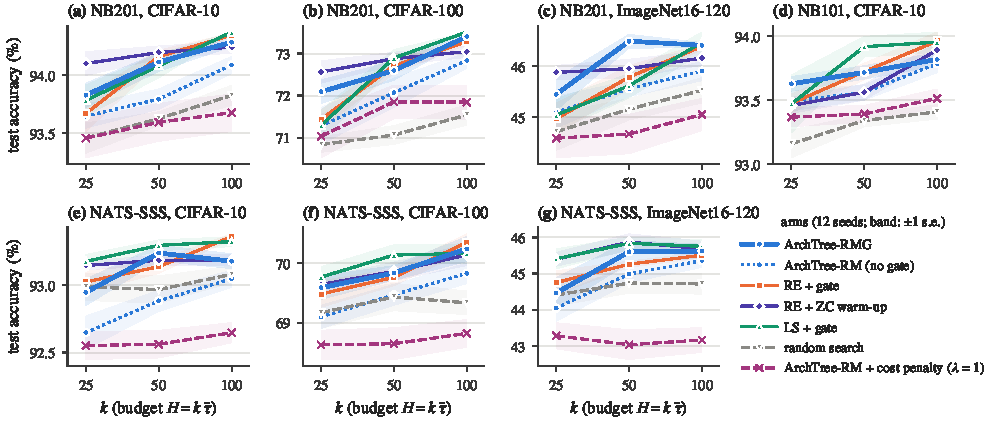
\includegraphics[width=\textwidth]{figs/fig8_equal_gpu_hours.pdf}
\caption{Test accuracy of the best-validation architecture found within an equal GPU-hour budget $H=k\bar\tau$ (mean $\pm$ standard error, 12 seeds). Solid lines use the label-free gate (or a ZC warm-up); dotted and dashed lines are ungated or cost-penalised. The gate raises the mean accuracy of every proposer, while a strong cost penalty ($\lambda=1$) lowers it on all seven benchmark--dataset pairs.}
\label{fig:egh}
\end{figure*}

\subsection{Equal GPU-hours}\label{sec:egh}

Comparisons at an equal number of proposals favour any method that evaluates fewer, but possibly more expensive, architectures. Figure~\ref{fig:egh} therefore gives every arm the same training budget $H_k$ (Eq.~\ref{eq:egh}). Across 13 comparison arms and up to 21 cells (seven benchmark--dataset pairs, three budgets), \algname{} with the label-free gate records 57 wins, 204 ties and \emph{no loss} (Holm within arm). The largest mean margins are over the cost-penalised gates ($+1.36$ points for random search and $+1.01$ for \algname-RM with $\lambda=1$; 15 and 16 wins) and over random search without the gate ($+0.67$, 10 wins); against ungated RE, LS and \algname-RM the margins are $+0.36$, $+0.16$ and $+0.38$ points with at most two wins each. The wins are concentrated against the cost-penalised gates and against random search with or without the gate; against RE and LS with the same gate, and against RE with zero-cost warm-up, all 21 cells are ties.


\begin{figure*}[t]
\centering
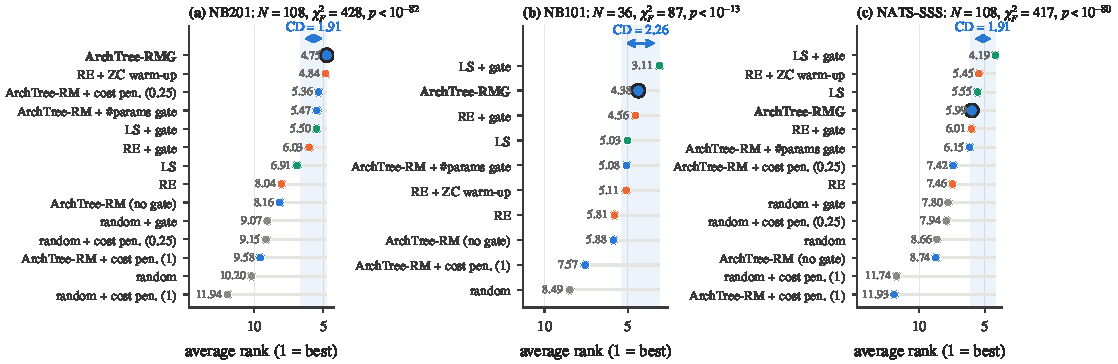
\includegraphics[width=\textwidth]{figs/fig9_ranks.pdf}
\caption{Average Friedman rank at equal GPU-hours (blocks = dataset $\times$ budget $\times$ seed; numbers give the rank). The shaded band spans the Nemenyi critical difference (CD) from the best arm; arms inside it are not significantly worse than the best. Colours mark the proposer family; \rmg{} (large marker) is inside the band on all three benchmarks.}
\label{fig:ranks}
\end{figure*}

Friedman ranks (Figure~\ref{fig:ranks}) give the same picture. On NAS-Bench-201 \algname{} has the lowest average rank (4.75), essentially tied with RE plus zero-cost warm-up (4.84; CD = 1.91). On NAS-Bench-101 it is second (4.38, behind LS with the gate at 3.11; CD = 2.26) and on NATS-Bench SSS fourth (5.99, behind LS with the gate at 4.19), in both cases within the CD; section~\ref{sec:stats} gives the per-run probabilities and equivalence tests.

Under the same label-free gate at a fixed proposal budget, \algname{} matches RE in all 12 NAS-Bench-201 cells while using 19--24\% fewer GPU-hours (55, 115 and 351 GPU-h against 72, 146 and 434 at budget 200) and has no loss in 240 same-gate comparisons against five proposers under four gates; section~\ref{sec:transfer} examines how well the gate itself transfers.

\begin{table}[t]
\caption{Gate-cost criterion (Eq.~\ref{eq:slope}) with normal-score correlations, and the measured effect of a $\lambda=1$ cost penalty on \algname{} at equal GPU-hours.}\label{tab:gatecost}
\centering\footnotesize
\setlength{\tabcolsep}{3.2pt}
\begin{tabular}{@{}llccccc@{}}
\toprule
Bench. & Data & $r_{PA}$ & $r_{PD}$ & $r_{DA}$ & Slope & Measured\\
\midrule
NB201 & C10 & 0.83 & 0.79 & 0.69 & $-0.04$ & 3 L / 0 T\\
NB201 & C100 & 0.86 & 0.79 & 0.72 & $-0.04$ & 1 L / 2 T\\
NB201 & IN16 & 0.82 & 0.79 & 0.66 & $-0.02$ & 2 L / 1 T\\
NB101 & C10 & 0.47 & 0.82 & 0.44 & $-0.05$ & 1 L / 2 T\\
NATS & C10 & 0.74 & 0.67 & 0.89 & $-0.39$ & 3 L / 0 T\\
NATS & C100 & 0.84 & 0.67 & 0.75 & $-0.18$ & 3 L / 0 T\\
NATS & IN16 & 0.83 & 0.67 & 0.85 & $-0.29$ & 3 L / 0 T\\
\bottomrule
\end{tabular}
\tablenotes{L/T: losses/ties of the penalised gate against the plain gate over $k\in\{25,50,100\}$ (Holm); no cell shows a win. NATS: NATS-Bench SSS.}
\end{table}

\begin{figure*}[t]
\centering
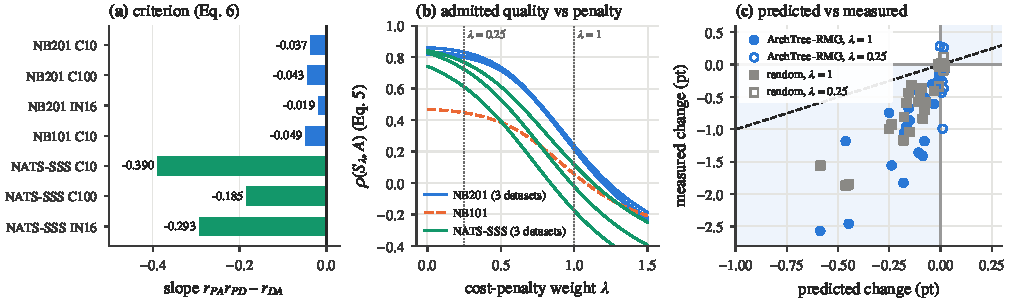
\includegraphics[width=\textwidth]{figs/fig10_gate_cost.pdf}
\caption{(a) Criterion slope $r_{PA}r_{PD}-r_{DA}$ for each benchmark--dataset pair; all are negative, predicting that a cost penalty hurts (blue: cell spaces; green: width space). (b) Correlation between the penalised gate score and accuracy as a function of $\lambda$ (Eq.~\ref{eq:corr}) with the fitted correlations; dotted lines mark the two penalties tested. (c) Predicted against measured change in test accuracy caused by a cost-penalised gate at equal GPU-hours (one point per benchmark, dataset and budget). Points in the shaded quadrants have the predicted sign; the pooled ordering, driven mainly by the gap between cell and width spaces, is well predicted, but measured losses are several times larger than predicted (dashed line: $y=x$).}
\label{fig:gatecost}
\end{figure*}

\subsection{Proxies and training cost}\label{sec:cost}

Figure~\ref{fig:proxies}(b) shows that, in the cell spaces, the label-free ensemble correlates strongly with training time (Spearman $\rho$ = 0.78 on NAS-Bench-201 and 0.63 on NAS-Bench-101, against 0.83 and 0.87 for parameter count; NASWOT alone 0.82). Accordingly, the top 35\% of NAS-Bench-201 architectures by proxy cost 1.22 times the mean to train. However, the truly best 35\% by validation accuracy cost 1.16--1.18 times the mean, because accuracy itself rises with network size, so the proxy over-pays by only 3--5\% relative to the truly best set (Figure~\ref{fig:design}(b)). In the width space of NATS-Bench SSS the ensemble is only weakly cost-related ($\rho$ = 0.20--0.21), whereas parameter count still is ($\rho$ = 0.68--0.74), and the proxy follows accuracy instead ($\rho$ = 0.73; Figure~\ref{fig:proxies}(d)). The components differ as well: SVD entropy is nearly cost-neutral (its top 35\% train 1.13 times the mean, below the 1.16 of the truly best 35\%), whereas NASWOT over-pays by 6\%. On NAS-Bench-101 the over-payment is much larger: the admitted 35\% train 1.35 times the mean against 1.14 for the truly best, so the gate saves less GPU time there than its evaluation savings suggest.

Table~\ref{tab:gatecost} applies the criterion of Eq.~(\ref{eq:slope}) to all seven benchmark--dataset pairs, using parameter count as the predicted cost $D$. The slope is negative everywhere, so a cost penalty is predicted to lower the quality of admitted architectures. The two regimes differ: in the cell spaces the slope is slightly negative ($-0.02$ to $-0.05$), because the proxy already tracks cost, whereas on NATS-Bench SSS it is strongly negative ($-0.18$ to $-0.39$), because accuracy is tightly coupled to width ($r_{DA}$ = 0.75--0.89). Figure~\ref{fig:gatecost}(b) shows what this means for the gate: as $\lambda$ grows, the correlation of the admitted score with accuracy falls monotonically on every pair, from 0.82--0.86 to 0.22--0.24 at $\lambda=1$ on NAS-Bench-201 and to between $-0.18$ and $+0.12$ on NATS-Bench SSS, where a gate with $\lambda=1$ is barely better than random. The measured outcome agrees (Figure~\ref{fig:gatecost}(c)). With $\lambda=1$, \algname{} is significantly worse than unpenalised in 16 of 21 cells and never better, and its change in test accuracy is negative in all 21 cells (random search with $\lambda=1$: 18 of 18). Over all penalised arms, predicted and measured changes share the same sign in 72\% (\algname) and 69\% (random) of cells, with Spearman correlations of $+0.78$ and $+0.86$. The copula simulation reproduces the level of the unpenalised gate closely (predicted 93.89, 71.96 and 45.67 against measured 93.92, 71.92 and 45.45 for gated random search on NAS-Bench-201 at $k=100$) but predicts losses several times smaller than those measured, so we use the criterion for its sign and ranking, not for magnitudes.


\begin{figure*}[t]
\centering
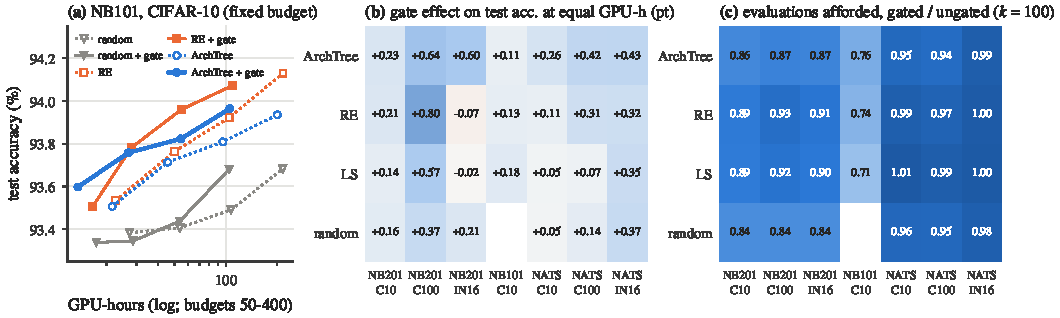
\includegraphics[width=\textwidth]{figs/fig15_transfer.pdf}
\caption{Transfer to NAS-Bench-101 and use of the gate with other proposers. (a) NAS-Bench-101: test accuracy against GPU-hours at budgets 50--400 for three proposers with (solid, filled) and without (dotted, open) the label-free gate (12 seeds). (b) Change in test accuracy at equal GPU-hours when the label-free gate is added to each proposer, averaged over $k\in\{25,50,100\}$ (blank: arm not run). (c) Ratio of real evaluations made within $H_{100}$ with and without the gate; values below 1 mean that the gate buys fewer, more expensive architectures.}
\label{fig:transfer}
\end{figure*}

\subsection{Transfer to NAS-Bench-101 and the gate on other proposers}\label{sec:transfer}

Figure~\ref{fig:transfer}(a) repeats the same-budget experiment on NAS-Bench-101 (576 runs) with three proposers and four gates. Proxies are weaker here, yet at budget 400 the label-free gate still removes 59\% of the real evaluations and 47\% of the GPU-hours, without losing accuracy against ungated \algname. Across 16 gate--budget cells, \algname{} beats random search in 14 and ties in 2. Against RE it ties in 15 and loses one (parameter-count gate, budget 100, $-0.31$ points). At budget 400 the label-free gate gives 93.96 for \algname, 94.07 for RE and 93.68 for random search with 163 real evaluations; RE is numerically 0.1--0.2 points ahead, and \algname's GPU-hour advantage over RE shrinks to about 4\% (105 against 110 GPU-h). Over the cost range they share, the gated curves lie above their ungated counterparts, so the gate saves cost without a detectable accuracy loss even where proxies rank poorly. This is consistent with the data (Table~\ref{tab:datastats}): accuracy is less coupled to cost in NAS-Bench-101 ($\rho$ = 0.34), so a cost-correlated proxy has less to offer.

Figure~\ref{fig:transfer}(b) shows what the gate does for other proposers at equal GPU-hours. With the gate, test accuracy is higher in 25 of 27 proposer--benchmark cells, by 0.38 points on average for \algname, 0.26 for RE, 0.22 for random search and 0.19 for LS; the two exceptions ($-0.07$ and $-0.02$, RE and LS on NAS-Bench-201 ImageNet16-120), like several small gains, are within seed noise, and the per-proposer gain was not tested for significance. Figure~\ref{fig:transfer}(c) shows how the gain is obtained. In the cell spaces the gate spends the same budget on 71--93\% as many evaluations, because the architectures it admits are larger; on NATS-Bench SSS it spends it on 94--101\% as many, because there the proxy is not cost-biased. Accuracy improves in both regimes, so the gain does not depend on the proxy's cost bias.


\begin{figure*}[t]
\centering
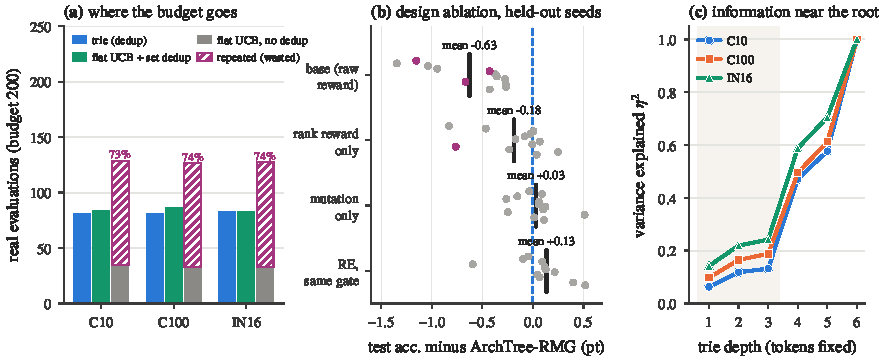
\includegraphics[width=\textwidth]{figs/fig11_ablations.pdf}
\caption{(a) Real evaluations at a budget of 200 proposals for the trie and for a flat UCB over positions, with or without deduplication; hatched segments are evaluations of already-trained architectures. (b) Held-out-seed design ablation: test accuracy of each variant minus \rmg{} in each of the 12 dataset--budget cells (dots; red marks cells where \rmg{} is significantly better after Holm correction) and the mean over cells (bar). (c) Share of the variance of NAS-Bench-201 validation accuracy explained by the first $d$ tokens; the shaded depths are where a tree would have to share statistics.}
\label{fig:ablation}
\end{figure*}

\subsection{Ablations: what the parts contribute}\label{sec:ablation}

\textit{Tree structure versus deduplication.} Replacing the trie by a flat bandit over the six positions (Figure~\ref{fig:ablation}(a)) shows where the benefit comes from. A flat bandit with no memory spends 73--74\% of its real evaluations at budget 200 on architectures it has already trained, and the trie beats it in 3 of 12 cells before and 1 after Holm correction ($+0.53$ points on average). With set-based deduplication added to the flat bandit, the difference falls to $+0.06$ points and 0 of 12 cells. We therefore detect no gain from the hierarchy beyond deduplication (equivalence untested). The landscape, which hierarchical optimistic search \cite{kocsis2006,bubeck2011,munos2011} assumes smooth, is consistent with this (Figure~\ref{fig:ablation}(c)): the first one to three tokens of a NAS-Bench-201 architecture explain only 6--24\% of the variance in accuracy ($\eta^2$), rising to 47--59\% at depth four, so statistics kept close to the root say little about unvisited leaves.

\textit{Design changes on held-out seeds.} On 12 seeds not used for any design decision (Figure~\ref{fig:ablation}(b)), \algname-base is 0.63 points worse than \rmg{} on average (significantly so in 3 of 12 cells), the rank reward alone is 0.18 points worse, mutation alone is level ($+0.03$), and RE with the same gate is level ($+0.13$, all ties), while \rmg{} needs 12--19\% fewer GPU-hours than RE at budget 200. The accuracy of \rmg{} thus comes mainly from its evolutionary step, while the trie and the gate reduce what that accuracy costs.


\begin{figure*}[t]
\centering
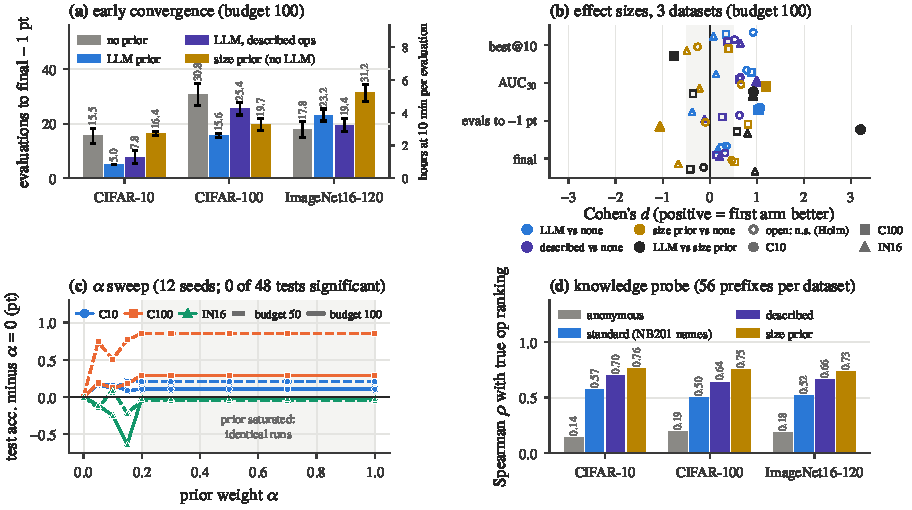
\includegraphics[width=\textwidth]{figs/fig12_llm.pdf}
\caption{LLM prior. (a) Real evaluations needed to come within one point of the best validation accuracy in the space (budget 100, mean $\pm$ standard error, 12 seeds); the right axis converts them to hours at 10 minutes per evaluation. The early trajectory under the LLM prior is the same for every seed, so its error bar is near zero. (b) Cohen's $d$ for four paired comparisons on four convergence metrics (best accuracy after 10 evaluations, area under the first 30 evaluations, evaluations to $-1$ point with the sign flipped so that faster is positive, and final accuracy); filled markers are significant after Holm correction, the grey band marks $|d|<0.5$. (c) Test accuracy relative to $\alpha=0$ in a sweep of the prior weight. (d) Spearman correlation between the operation ranking proposed by the prior and the true NAS-Bench-201 ranking over 56 trie prefixes; 0 is chance.}
\label{fig:llm}
\end{figure*}

\subsection{What does the LLM prior add?}\label{sec:llm}

With the prior enabled ($\alpha=0.3$), the search comes within one point of the best validation accuracy in the space after 5.0 instead of 15.5 evaluations on CIFAR-10 and 15.6 instead of 30.8 on CIFAR-100 ($p_{\mathrm{Holm}}=0.047$ in both cases, Cohen's $d\approx1.0$, although on CIFAR-10 the prior's trajectory is identical for all seeds; Figure~\ref{fig:llm}(a), (b)). At ten minutes per evaluation this is 0.8 instead of 2.6 hours on CIFAR-10; the model's own response time is negligible next to a single evaluation. On ImageNet16-120 the prior is not faster (23.2 against 17.8 evaluations, not significant). The effect is confined to the start of the search: on final accuracy every comparison is a tie, and against no prior $|d|<0.36$ (Figure~\ref{fig:llm}(b)). The sweep of $\alpha$ (Figure~\ref{fig:llm}(c); budgets 50 and 100, 12 seeds) points the same way. At $\alpha\ge0.2$ the prior saturates and the runs become identical; at that level it changes test accuracy by $+0.85$ and $+0.29$ points on CIFAR-100, $+0.21$ and $+0.11$ on CIFAR-10 and $-0.05$ and $-0.02$ on ImageNet16-120 (budget 50 and 100). None of the 48 tests is significant after Holm correction. A larger model (\texttt{gpt-oss-120b}) ranks operations slightly better ($\rho$ = 0.61 against 0.60) but does not search better.

Three controls address what the model knows (Figure~\ref{fig:llm}(d)). When operation names are replaced by arbitrary labels, the model's ranking of operations is only slightly better than chance ($\rho$ = 0.14--0.19; significant but small, $d$ = 0.3--0.4). When the operations are described in plain words without NAS-Bench-201 names, the ranking is \emph{better} than with the benchmark's own names ($\rho$ = 0.64--0.70 against 0.50--0.57), which argues against recall of memorised benchmark tables. A knowledge-free prior that scores operations by their size ranks single operations best of all ($\rho$ = 0.73--0.76), yet it searches worse: it is no faster than no prior on CIFAR-10 and is significantly slower on ImageNet16-120 ($+13.5$ evaluations, $p_{\mathrm{Holm}}=0.018$), whereas the LLM prior is faster than the size prior on CIFAR-10 ($p_{\mathrm{Holm}}=0.003$, $d=4.0$) and has a larger area under the early curve on CIFAR-10 and ImageNet16-120 ($d$ = 0.93 and 0.92, both significant). The LLM thus appears to add more than a size rule early, though one deterministic trajectory limits this inference.


\begin{figure*}[t]
\centering
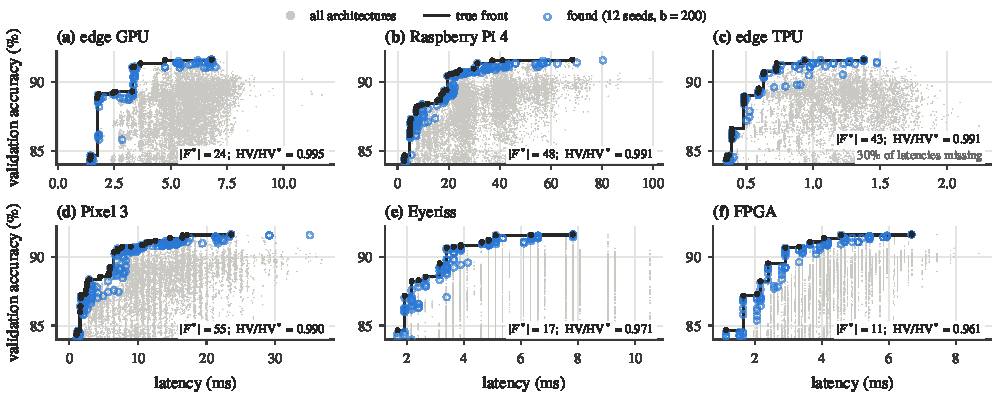
\includegraphics[width=\textwidth]{figs/fig13_hw_fronts.pdf}
\caption{Accuracy--latency trade-off on the six HW-NAS-Bench devices (CIFAR-10, architectures above 84\% validation accuracy). Grey: all architectures; black: exact Pareto front of the 15,625 architectures; blue circles: members of the fronts found by \algname-HW at a budget of 200 (union over 12 seeds). The device determines both the shape of the front and which cells lie on it.}
\label{fig:hwfronts}
\end{figure*}

\subsection{Hardware-aware search}\label{sec:hw}

The equal-GPU-hour study measures the cost of \emph{finding} a network; on an edge device, the cost that matters is the latency of \emph{running} it. HW-NAS-Bench tests whether the loop extends to a second objective on the same 15,625 cells and whether a front searched for one device helps on another. A latency-penalised trie search is compared with random and NSGA-II-style search. It uses rank-normalised UCB with max backup on the reward $A-5\min(\ell/50\,\mathrm{ms},1)$, where $\ell$ is the latency, and has no gate and no mutation, so that the objective alone is changed; it is denoted \algname-HW. The comparison runs at budgets 25--200 (864 runs) using hypervolume (HV) \cite{zitzler1999} and inverted generational distance (IGD) against the exact fronts.

\begin{table}[t]
\caption{Accuracy--latency search on HW-NAS-Bench at budget 200 (CIFAR-10, mean of 12 seeds).}\label{tab:hw}
\centering\footnotesize
\setlength{\tabcolsep}{1.6pt}
\begin{tabular}{@{}lccccc@{}}
\toprule
Device & HV ($\times10^3$) & IGD & $|F|$ & $|F^{*}|$ & HV / HV$^{*}$\\
 & AT / Rnd / NSGA & AT / Rnd / NSGA & AT & & AT\\
\midrule
Edge GPU & 91.35 / 91.06 / 91.18 & 0.22 / 0.38 / 0.17 & 12.6 & 24 & 0.995\\
RPi 4 & 91.00 / 90.88 / 91.16 & 2.04 / 1.31 / 1.78 & 18.4 & 48 & 0.991\\
Edge TPU & 91.38 / 91.16 / 91.40 & 0.22 / 0.26 / 0.15 & 13.3 & 43 & 0.991\\
Pixel 3 & 91.24 / 91.05 / 91.25 & 0.69 / 0.80 / 1.44 & 18.0 & 55 & 0.990\\
Eyeriss & 91.33 / 91.03 / 91.26 & 0.51 / 0.64 / 0.34 & 11.0 & 17 & 0.971\\
FPGA & 91.40 / 91.07 / 91.30 & 0.55 / 0.64 / 0.35 & 11.1 & 11 & 0.961\\
\bottomrule
\end{tabular}
\tablenotes{AT: \algname-HW (latency-penalised trie search, no gate); Rnd: random; NSGA: NSGA-II-style. $|F|$: size of the found front; $|F^{*}|$: size of the true front; HV/HV$^{*}$: share of the attainable hypervolume. All 96 HV and IGD comparisons (6 devices, 4 budgets, 2 rivals, 2 metrics) are ties after Holm correction.}
\end{table}

\begin{figure*}[t]
\centering
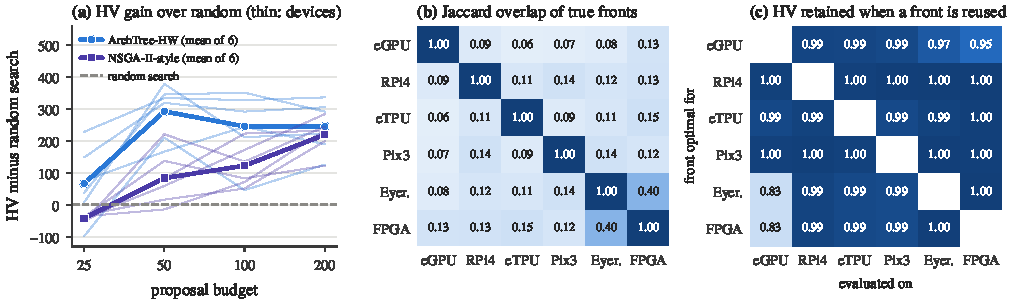
\includegraphics[width=\textwidth]{figs/fig14_hw_summary.pdf}
\caption{(a) Hypervolume of \algname-HW and NSGA-II-style search minus that of random search (thin lines: the six devices; thick: their mean; 12 seeds). (b) Jaccard overlap between the true Pareto fronts of each pair of devices. (c) Share of a device's attainable hypervolume that is retained when the true front of another device is used instead (row: device the front is optimal for; column: device it is evaluated on).}
\label{fig:hwsum}
\end{figure*}

The found fronts lie close to the true fronts (Figure~\ref{fig:hwfronts}) and attain 96--99.5\% of the best possible hypervolume at budget 200, up from 85--94\% at budget 25. We call this share HV/HV$^{*}$ the \emph{hardware-aware coverage} of a search: the fraction of the best achievable accuracy--latency trade-off that its front attains. The fronts are not, however, clearly better than those of the simple rivals (Table~\ref{tab:hw}): all 96 comparisons are ties after Holm correction. Figure~\ref{fig:hwsum}(a) shows why. \algname-HW is ahead of random search from the smallest budget, by 70 to 290 hypervolume units on average, and NSGA-II-style search catches up by budget 200. The found fronts are also sparse: only 2--5\% of the true front members are found, because 200 proposals sample about 1.3\% of the space.

The more useful finding concerns the devices themselves. The true Pareto fronts barely overlap (mean Jaccard index 0.13, at most 0.40 between Eyeriss and FPGA; Figure~\ref{fig:hwsum}(b)), and only one among the 15,625 architectures lies on the Pareto front of all six devices. Even so, a front that is optimal for one device retains 98\% of the attainable hypervolume on another on average (Figure~\ref{fig:hwsum}(c); worst case 83\%, Eyeriss or FPGA to edge GPU). By these measures a front searched for one device is a reasonable start for another, even though its members are rarely optimal there.

\subsection{Overview of the statistical evidence}\label{sec:stats}

\begin{table}[t]
\caption{All paired tests of the study by family: number of tests, tests with $p<0.05$ before correction, tests significant after Holm correction (families as in the note), and the direction of the significant results.}\label{tab:allstats}
\centering\footnotesize
\setlength{\tabcolsep}{2pt}
\begin{tabular}{@{}>{\raggedright\arraybackslash}p{0.34\columnwidth}rrr>{\raggedright\arraybackslash}p{0.3\columnwidth}@{}}
\toprule
Family & Tests & Raw & Holm & Significant results\\
\midrule
Fixed budget vs 9 baselines & 108 & 38 & 20 & 20 RMG wins\\
Same gate, 5 proposers & 240 & 100 & 47 & 47 ArchTree wins\\
Equal GPU-hours, 3 benchmarks & 261 & 96 & 57 & 57 RMG wins\\
NB101, same gate & 32 & 16 & 15 & 14 wins, 1 loss (RE)\\
NB101, equal evaluations & 36 & 13 & 11 & 11 ArchTree wins\\
Held-out design ablation & 48 & 10 & 4 & all favour RMG\\
Trie vs flat bandit & 24 & 3 & 1 & trie better\\
Proxy subsets & 48 & 6 & 2 & SVD entropy alone worse\\
UCB $C$ and backup & 78 & 9 & 0 & --\\
$\alpha$ sweep & 48 & 11 & 0 & --\\
LLM convergence (12 metrics) & 360 & 149 & 109 & 53 early; 23 LLM time; 33 rescaled\\
LLM knowledge probe & 21 & 21 & 21 & all priors above chance\\
LLM model size & 4 & 1 & 0 & --\\
Hardware HV / IGD & 96 & 22 & 0 & --\\
\midrule
Total & 1,404 & 495 & 287 & \\
\bottomrule
\end{tabular}
\tablenotes{Raw: $p<0.05$ without correction. Holm: within the family as defined in section~\ref{sec:setup} (within baseline, arm or comparison). $\alpha$ sweep: 24 distinct tests (3 raw; runs with $\alpha\ge0.2$ coincide).}
\end{table}


\begin{figure*}[t]
\centering
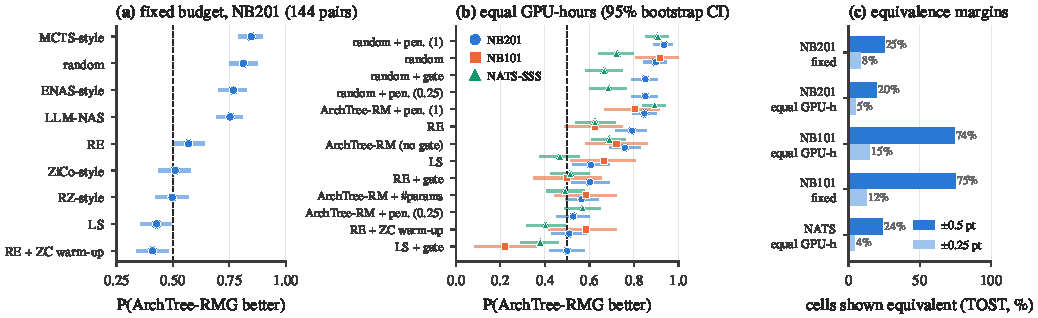
\includegraphics[width=\textwidth]{figs/fig16_stats.pdf}
\caption{Probability that \rmg{} finds a better architecture than another method on a paired (cell, seed) run, with stratified-bootstrap 95\% confidence intervals: (a) against the nine baselines at a fixed proposal budget on NAS-Bench-201; (b) against every arm at equal GPU-hours on the three benchmarks; the dashed line marks 0.5. (c) Share of cells in which two one-sided tests establish equivalence of \rmg{} with the other arms within $\pm$0.5 and $\pm$0.25 points.}
\label{fig:stats}
\end{figure*}

Table~\ref{tab:allstats} collects the 1,404 paired tests of the study. Of the 677 tests in which \rmg{} is compared with another search method (first five rows), 149 are significant wins after Holm correction and one is a loss, so the direction is consistent, although against the strongest arms all corrected results are ties. The three sensitivity families (UCB setting, $\alpha$, proxy subsets; 174 tests) yield two significant results, so no setting has a detectable effect, and all 96 hardware tests are ties. The significant LLM results all concern early-search speed, never final accuracy. Friedman tests reject equal performance in every comparison ($p<10^{-7}$).

Figure~\ref{fig:stats} adds the per-run view. Against MCTS-style search, random search, ENAS-style search and LLM-NAS, \rmg{} wins 75--85\% of paired runs. Against RE, ZiCo-style and RZ-style search the probability is close to 0.5, and against LS and RE with ZC warm-up it is slightly below (0.43 and 0.41): these two methods win a few more paired runs at a fixed budget, although never significantly after correction and at 2.2--2.3 times the GPU-hours. At equal GPU-hours the intervals lie above 0.5 on NAS-Bench-201 against every random-search arm, the ungated arms and the $\lambda=1$ penalty, whereas LS with the gate is the stronger arm on NAS-Bench-101 (0.22) and NATS-Bench SSS (0.38), and RE with ZC warm-up on NATS-Bench SSS (0.40). Within $\pm$0.5 points TOST confirms it in 20--25\% of the NAS-Bench-201 and NATS-Bench SSS cells and in about three quarters of the NAS-Bench-101 cells, and within $\pm$0.25 points in at most 15\%.

%% =====================================================================
\section{Discussion}\label{sec:discussion}

Deduplication is cheap and removes up to 75\% wasted evaluations for memoryless proposers, but a hash set provides it as well as a trie does. The label-free gate is the principal source of savings, and at equal GPU-hours it raised the mean accuracy of all four proposers we tried. Its bias towards large networks is real but mostly harmless, because accuracy is itself correlated with size; the criterion of Eq.~(\ref{eq:slope}) turns this observation into a test that can be run on a sample of architectures before committing a search budget. For a practitioner, the recipe is to estimate $r_{PA}$, $r_{PD}$ and $r_{DA}$ on a labelled sample of architectures; if $r_{PA}r_{PD}-r_{DA}<0$, the proxy gate should be used without a cost penalty.

\textit{Threats to validity.} \emph{Internal validity}: all methods share one code base, one data store and the same seeds, and test accuracy is never used for any decision; the \rmg{} design and the pass rate were selected using the main seeds and labelled NAS-Bench-201 data, so NAS-Bench-101, NATS-Bench SSS and 12 held-out seeds serve as out-of-sample tests. \emph{Construct validity}: GPU-hours are the training times recorded in the benchmark rather than times measured on our hardware, and the proxy network sees CIFAR-10 images for every dataset. \emph{Statistical conclusion validity}: twelve seeds detect differences of some tenths of a point but seldom prove equivalence within $\pm$0.5 points, and many comparisons are corrected for multiplicity, which favours ties; we therefore also report effect sizes, bootstrap probabilities and TOST. \emph{External validity}: all experiments use tabular benchmarks with image classification on small images; NAS-Bench-101 covers one dataset and was run without the LLM prior or hardware data, and HW-NAS-Bench lacks edge-TPU latencies for about 30\% of the cells. Finally, the LLM may have seen NAS-Bench-201 during pre-training; the described-operation control speaks against plain recall but cannot rule out all exposure.

%% =====================================================================
\section{Conclusions}\label{sec:conclusions}

We studied a NAS loop that never trains an architecture twice and trains only those proposals that a label-free zero-cost gate places in its top 35\%. Compared at equal GPU-hours on three benchmarks, it has no Holm-significant loss to any of 13 alternatives and stays within the critical difference of the best, while the gate alone roughly halves the training cost of a search with no significant accuracy loss and, at equal GPU-hours, raises the mean accuracy of every proposer it was added to. Zero-cost proxies track training cost in cell-based spaces, though not in a width space, and a simple criterion, $r_{PA}r_{PD}-r_{DA}$, was negative on all seven benchmark--dataset pairs, where a strong cost penalty did hurt; a pair with a positive slope remains to be tested. An LLM prior speeds up early search, but neither it nor the tree structure improves final accuracy; the next test is real training on larger spaces.

%% =====================================================================
\begin{nomenclature}
\nom{$\mathcal{A}$}{search space of architectures}
\nom{$a=(o_1,\dots,o_L)$}{architecture as a token sequence of length $L$}
\nom{$A(a)$, $T(a)$}{validation and test accuracy (\%)}
\nom{$\tau(a)$, $\bar\tau$}{training time of $a$; mean training time}
\nom{$H_k$}{GPU-hour budget, $k\bar\tau$}
\nom{$C$}{UCB exploration constant}
\nom{$r_t$}{rank-normalised reward}
\nom{$E$, $S$, $T$}{SVD entropy, SynFlow and NASWOT scores}
\nom{$z(\cdot)$}{standardised score}
\nom{$P(a)$}{label-free gate score}
\nom{$q$}{gate pass rate (0.35)}
\nom{$D$}{predicted cost, $\log(1+\#\text{params})$}
\nom{$\lambda$}{cost-penalty weight}
\nom{$r_{XY}$}{normal-score correlation of $X$ and $Y$}
\nom{$\alpha$, $\alpha_t$}{LLM prior weight and its decayed value}
\nom{$\tau$, $\rho$}{Kendall and Spearman rank correlations}
\nom{$S_\lambda$}{cost-penalised gate score}
\nom{$\eta^2$}{share of accuracy variance explained by a prefix}
\end{nomenclature}

\appendix
\renewcommand{\thesection}{Appendix \Alph{section}.}
\section{Derivation of the gate-cost criterion}\label{app:derivation}

Let $Z_P$, $Z_D$ and $Z_A$ be standard normal scores of the proxy, the predicted cost and accuracy, with correlations $r_{PD}$, $r_{PA}$ and $r_{DA}$. For $S_\lambda=Z_P-\lambda Z_D$,
\begin{align}
\operatorname{Cov}(S_\lambda,Z_A)&=r_{PA}-\lambda r_{DA},\\
\operatorname{Var}(S_\lambda)&=1+\lambda^{2}-2\lambda r_{PD},
\end{align}
which gives Eq.~(\ref{eq:corr}). Writing $g(\lambda)=r_{PA}-\lambda r_{DA}$ and $h(\lambda)=1+\lambda^2-2\lambda r_{PD}$,
\begin{equation}
\frac{\partial\rho}{\partial\lambda}=\frac{g'(\lambda)}{\sqrt{h(\lambda)}}-\frac{g(\lambda)\,h'(\lambda)}{2\,h(\lambda)^{3/2}}.
\end{equation}
At $\lambda=0$, $g=r_{PA}$, $g'=-r_{DA}$, $h=1$ and $h'=-2r_{PD}$, so the slope equals $-r_{DA}+r_{PA}r_{PD}$, which is Eq.~(\ref{eq:slope}). Because a threshold gate admits the upper tail of $S_\lambda$, a higher $\rho(S_\lambda,A)$ means higher expected accuracy among admitted architectures for a fixed pass rate under the Gaussian model.

%% =====================================================================
\section*{Acknowledgements}
The authors thank the Department of Computer Engineering and Technology, MIT World Peace University, Pune, for computing facilities, and the maintainers of NAS-Bench-101, NAS-Bench-201, NATS-Bench and HW-NAS-Bench for making their benchmarks public.

\section*{Declarations}
\textit{Funding.} No external funding was received for this work.\\
\textit{Competing interests.} The authors declare no competing interests.\\
\textit{Supplementary material.} Tables S1--S43 and Figures S1--S16 give the per-cell results and tests in detail.\\
\textit{Data and code availability.} All benchmarks are public. The code, configuration, seeds, result tables and a reproducibility bundle (environment, package versions and data checksums) are available at \url{https://github.com/Imaadhajwane/Arch-Tree-LLM}.\\
\textit{Use of AI-assisted tools.} The open-weight language models gpt-oss-20b and gpt-oss-120b \cite{openai2025gptoss} are objects of study in this work (sections~\ref{sec:method} and \ref{sec:llm}). Separately, the authors used Claude (Anthropic, Claude Opus 5.5) for coding assistance on the experiment and plotting scripts, for drafting and language editing of the manuscript, and for cross-checking reported numbers against the result files. No data or results were generated or altered by an AI tool; every figure was plotted directly from the result files. The authors reviewed all text and analyses and take full responsibility for the content.

\balance

\begin{thebibliography}{99}
\bibitem{zoph2017} Zoph B and Le Q V 2017 Neural architecture search with reinforcement learning. In: \textit{Proceedings of the International Conference on Learning Representations (ICLR)}

\bibitem{elsken2019} Elsken T, Metzen J H and Hutter F 2019 Neural architecture search: A survey. \textit{J. Mach. Learn. Res.} 20: 1--21

\bibitem{ren2021} Ren P, Xiao Y, Chang X, Huang P Y, Li Z, Chen X and Wang X 2021 A comprehensive survey of neural architecture search: Challenges and solutions. \textit{ACM Comput. Surv.} 54: 1--34

\bibitem{real2017} Real E, Moore S, Selle A, Saxena S, Suematsu Y L, Tan J et al. 2017 Large-scale evolution of image classifiers. In: \textit{Proceedings of the International Conference on Machine Learning (ICML)}, pp. 2902--2911

\bibitem{pham2018} Pham H, Guan M, Zoph B, Le Q and Dean J 2018 Efficient neural architecture search via parameter sharing. In: \textit{Proceedings of the International Conference on Machine Learning (ICML)}, pp. 4095--4104

\bibitem{liu2019} Liu H, Simonyan K and Yang Y 2019 DARTS: Differentiable architecture search. In: \textit{Proceedings of the International Conference on Learning Representations (ICLR)}

\bibitem{ying2019} Ying C, Klein A, Christiansen E, Real E, Murphy K and Hutter F 2019 NAS-Bench-101: Towards reproducible neural architecture search. In: \textit{Proceedings of the International Conference on Machine Learning (ICML)}, pp. 7105--7114

\bibitem{dong2020} Dong X and Yang Y 2020 NAS-Bench-201: Extending the scope of reproducible neural architecture search. In: \textit{Proceedings of the International Conference on Learning Representations (ICLR)}

\bibitem{dong2022} Dong X, Liu L, Musial K and Gabrys B 2022 NATS-Bench: Benchmarking NAS algorithms for architecture topology and size. \textit{IEEE Trans. Pattern Anal. Mach. Intell.} 44: 3634--3646

\bibitem{abdelfattah2021} Abdelfattah M S, Mehrotra A, Dudziak \L{} and Lane N D 2021 Zero-cost proxies for lightweight NAS. In: \textit{Proceedings of the International Conference on Learning Representations (ICLR)}

\bibitem{mellor2021} Mellor J, Turner J, Storkey A and Crowley E J 2021 Neural architecture search without training. In: \textit{Proceedings of the International Conference on Machine Learning (ICML)}, pp. 7588--7598

\bibitem{tanaka2020} Tanaka H, Kunin D, Yamins D L K and Ganguli S 2020 Pruning neural networks without any data by iteratively conserving synaptic flow. \textit{Adv. Neural Inf. Process. Syst.} 33: 6377--6389

\bibitem{krishnakumar2022} Krishnakumar A, White C, Zela A, Tu R, Safari M and Hutter F 2022 NAS-Bench-Suite-Zero: Accelerating research on zero cost proxies. \textit{Adv. Neural Inf. Process. Syst.} 35: 28037--28051

\bibitem{li2021hw} Li C, Yu Z, Fu Y, Zhang Y, Zhao Y, You H et al. 2021 HW-NAS-Bench: Hardware-aware neural architecture search benchmark. In: \textit{Proceedings of the International Conference on Learning Representations (ICLR)}

\bibitem{real2019} Real E, Aggarwal A, Huang Y and Le Q V 2019 Regularized evolution for image classifier architecture search. In: \textit{Proceedings of the AAAI Conference on Artificial Intelligence} 33, pp. 4780--4789

\bibitem{white2021bananas} White C, Neiswanger W and Savani Y 2021 BANANAS: Bayesian optimization with neural architectures for neural architecture search. In: \textit{Proceedings of the AAAI Conference on Artificial Intelligence} 35, pp. 10293--10301

\bibitem{li2020random} Li L and Talwalkar A 2020 Random search and reproducibility for neural architecture search. In: \textit{Proceedings of the Conference on Uncertainty in Artificial Intelligence (UAI)}, pp. 367--377

\bibitem{yang2020} Yang A, Esperan\c{c}a P M and Carlucci F M 2020 NAS evaluation is frustratingly hard. In: \textit{Proceedings of the International Conference on Learning Representations (ICLR)}

\bibitem{white2021ls} White C, Nolen S and Savani Y 2021 Exploring the loss landscape in neural architecture search. In: \textit{Proceedings of the Conference on Uncertainty in Artificial Intelligence (UAI)}, pp. 654--664

\bibitem{white2023} White C, Safari M, Sukthanker R, Ru B, Elsken T, Zela A et al. 2023 Neural architecture search: Insights from 1000 papers. arXiv:2301.08727

\bibitem{wang2020alphax} Wang L, Zhao Y, Jinnai Y, Tian Y and Fonseca R 2020 Neural architecture search using deep neural networks and Monte Carlo tree search. In: \textit{Proceedings of the AAAI Conference on Artificial Intelligence} 34, pp. 9983--9991

\bibitem{wang2019lanas} Wang L, Xie S, Li T, Fonseca R and Tian Y 2019 Sample-efficient neural architecture search by learning action space. arXiv:1906.06832

\bibitem{qian2022} Qian G, Zhang X, Li G, Zhao C, Chen Y, Zhang X et al. 2022 When NAS meets trees: An efficient algorithm for neural architecture search. In: \textit{Proceedings of the IEEE/CVF Conference on Computer Vision and Pattern Recognition Workshops}, pp. 2781--2786

\bibitem{lee2019} Lee N, Ajanthan T and Torr P H S 2019 SNIP: Single-shot network pruning based on connection sensitivity. In: \textit{Proceedings of the International Conference on Learning Representations (ICLR)}

\bibitem{li2023zico} Li G, Yang Y, Bhardwaj K and Marculescu R 2023 ZiCo: Zero-shot NAS via inverse coefficient of variation on gradients. In: \textit{Proceedings of the International Conference on Learning Representations (ICLR)}

\bibitem{zheng2023genius} Zheng M, Su X, You S, Wang F, Qian C, Xu C et al. 2023 Can GPT-4 perform neural architecture search? arXiv:2304.10970

\bibitem{chen2023evoprompt} Chen A, Dohan D M and So D R 2023 EvoPrompting: Language models for code-level neural architecture search. \textit{Adv. Neural Inf. Process. Syst.} 36

\bibitem{nasir2024llmatic} Nasir M U, Earle S, Cleghorn C, James S and Togelius J 2024 LLMatic: Neural architecture search via large language models and quality diversity optimization. In: \textit{Proceedings of the Genetic and Evolutionary Computation Conference (GECCO)}. https://doi.org/10.1145/3638529.3654017

\bibitem{roy2007} Roy O and Vetterli M 2007 The effective rank: A measure of effective dimensionality. In: \textit{Proceedings of the European Signal Processing Conference (EUSIPCO)}, pp. 606--610

\bibitem{krizhevsky2009} Krizhevsky A 2009 Learning multiple layers of features from tiny images. Technical report, University of Toronto, Toronto

\bibitem{chrabaszcz2017} Chrabaszcz P, Loshchilov I and Hutter F 2017 A downsampled variant of ImageNet as an alternative to the CIFAR datasets. arXiv:1707.08819

\bibitem{openai2025gptoss} OpenAI 2025 gpt-oss-120b \& gpt-oss-20b model card. arXiv:2508.10925

\bibitem{deb2002} Deb K, Pratap A, Agarwal S and Meyarivan T 2002 A fast and elitist multiobjective genetic algorithm: NSGA-II. \textit{IEEE Trans. Evol. Comput.} 6: 182--197

\bibitem{wilcoxon1945} Wilcoxon F 1945 Individual comparisons by ranking methods. \textit{Biometrics Bull.} 1: 80--83

\bibitem{holm1979} Holm S 1979 A simple sequentially rejective multiple test procedure. \textit{Scand. J. Stat.} 6: 65--70

\bibitem{demsar2006} Dem\v{s}ar J 2006 Statistical comparisons of classifiers over multiple data sets. \textit{J. Mach. Learn. Res.} 7: 1--30

\bibitem{schuirmann1987} Schuirmann D J 1987 A comparison of the two one-sided tests procedure and the power approach for assessing the equivalence of average bioavailability. \textit{J. Pharmacokinet. Biopharm.} 15: 657--680

\bibitem{agarwal2021} Agarwal R, Schwarzer M, Castro P S, Courville A and Bellemare M G 2021 Deep reinforcement learning at the edge of the statistical precipice. \textit{Adv. Neural Inf. Process. Syst.} 34: 29304--29320

\bibitem{kendall1938} Kendall M G 1938 A new measure of rank correlation. \textit{Biometrika} 30: 81--93

\bibitem{chen2021drnas} Chen X, Wang R, Cheng M, Tang X and Hsieh C J 2021 DrNAS: Dirichlet neural architecture search. In: \textit{Proceedings of the International Conference on Learning Representations (ICLR)}

\bibitem{chen2021tenas} Chen W, Gong X and Wang Z 2021 Neural architecture search on ImageNet in four GPU hours: A theoretically inspired perspective. In: \textit{Proceedings of the International Conference on Learning Representations (ICLR)}

\bibitem{kocsis2006} Kocsis L and Szepesv\'{a}ri C 2006 Bandit based Monte-Carlo planning. In: \textit{Proceedings of the European Conference on Machine Learning (ECML)}, pp. 282--293

\bibitem{bubeck2011} Bubeck S, Munos R, Stoltz G and Szepesv\'{a}ri C 2011 X-armed bandits. \textit{J. Mach. Learn. Res.} 12: 1655--1695

\bibitem{munos2011} Munos R 2011 Optimistic optimization of a deterministic function without the knowledge of its smoothness. \textit{Adv. Neural Inf. Process. Syst.} 24: 783--791

\bibitem{zitzler1999} Zitzler E and Thiele L 1999 Multiobjective evolutionary algorithms: A comparative case study and the strength Pareto approach. \textit{IEEE Trans. Evol. Comput.} 3: 257--271

\end{thebibliography}

\end{document}
